\chapter{FOCUS ON NORTH AFRICA}

\section{Temperature}

\subsection{Deterministic evaluation results}
\subsubsection{\textbf{Correlation}}


\begin{figure}[H]
    \centering
    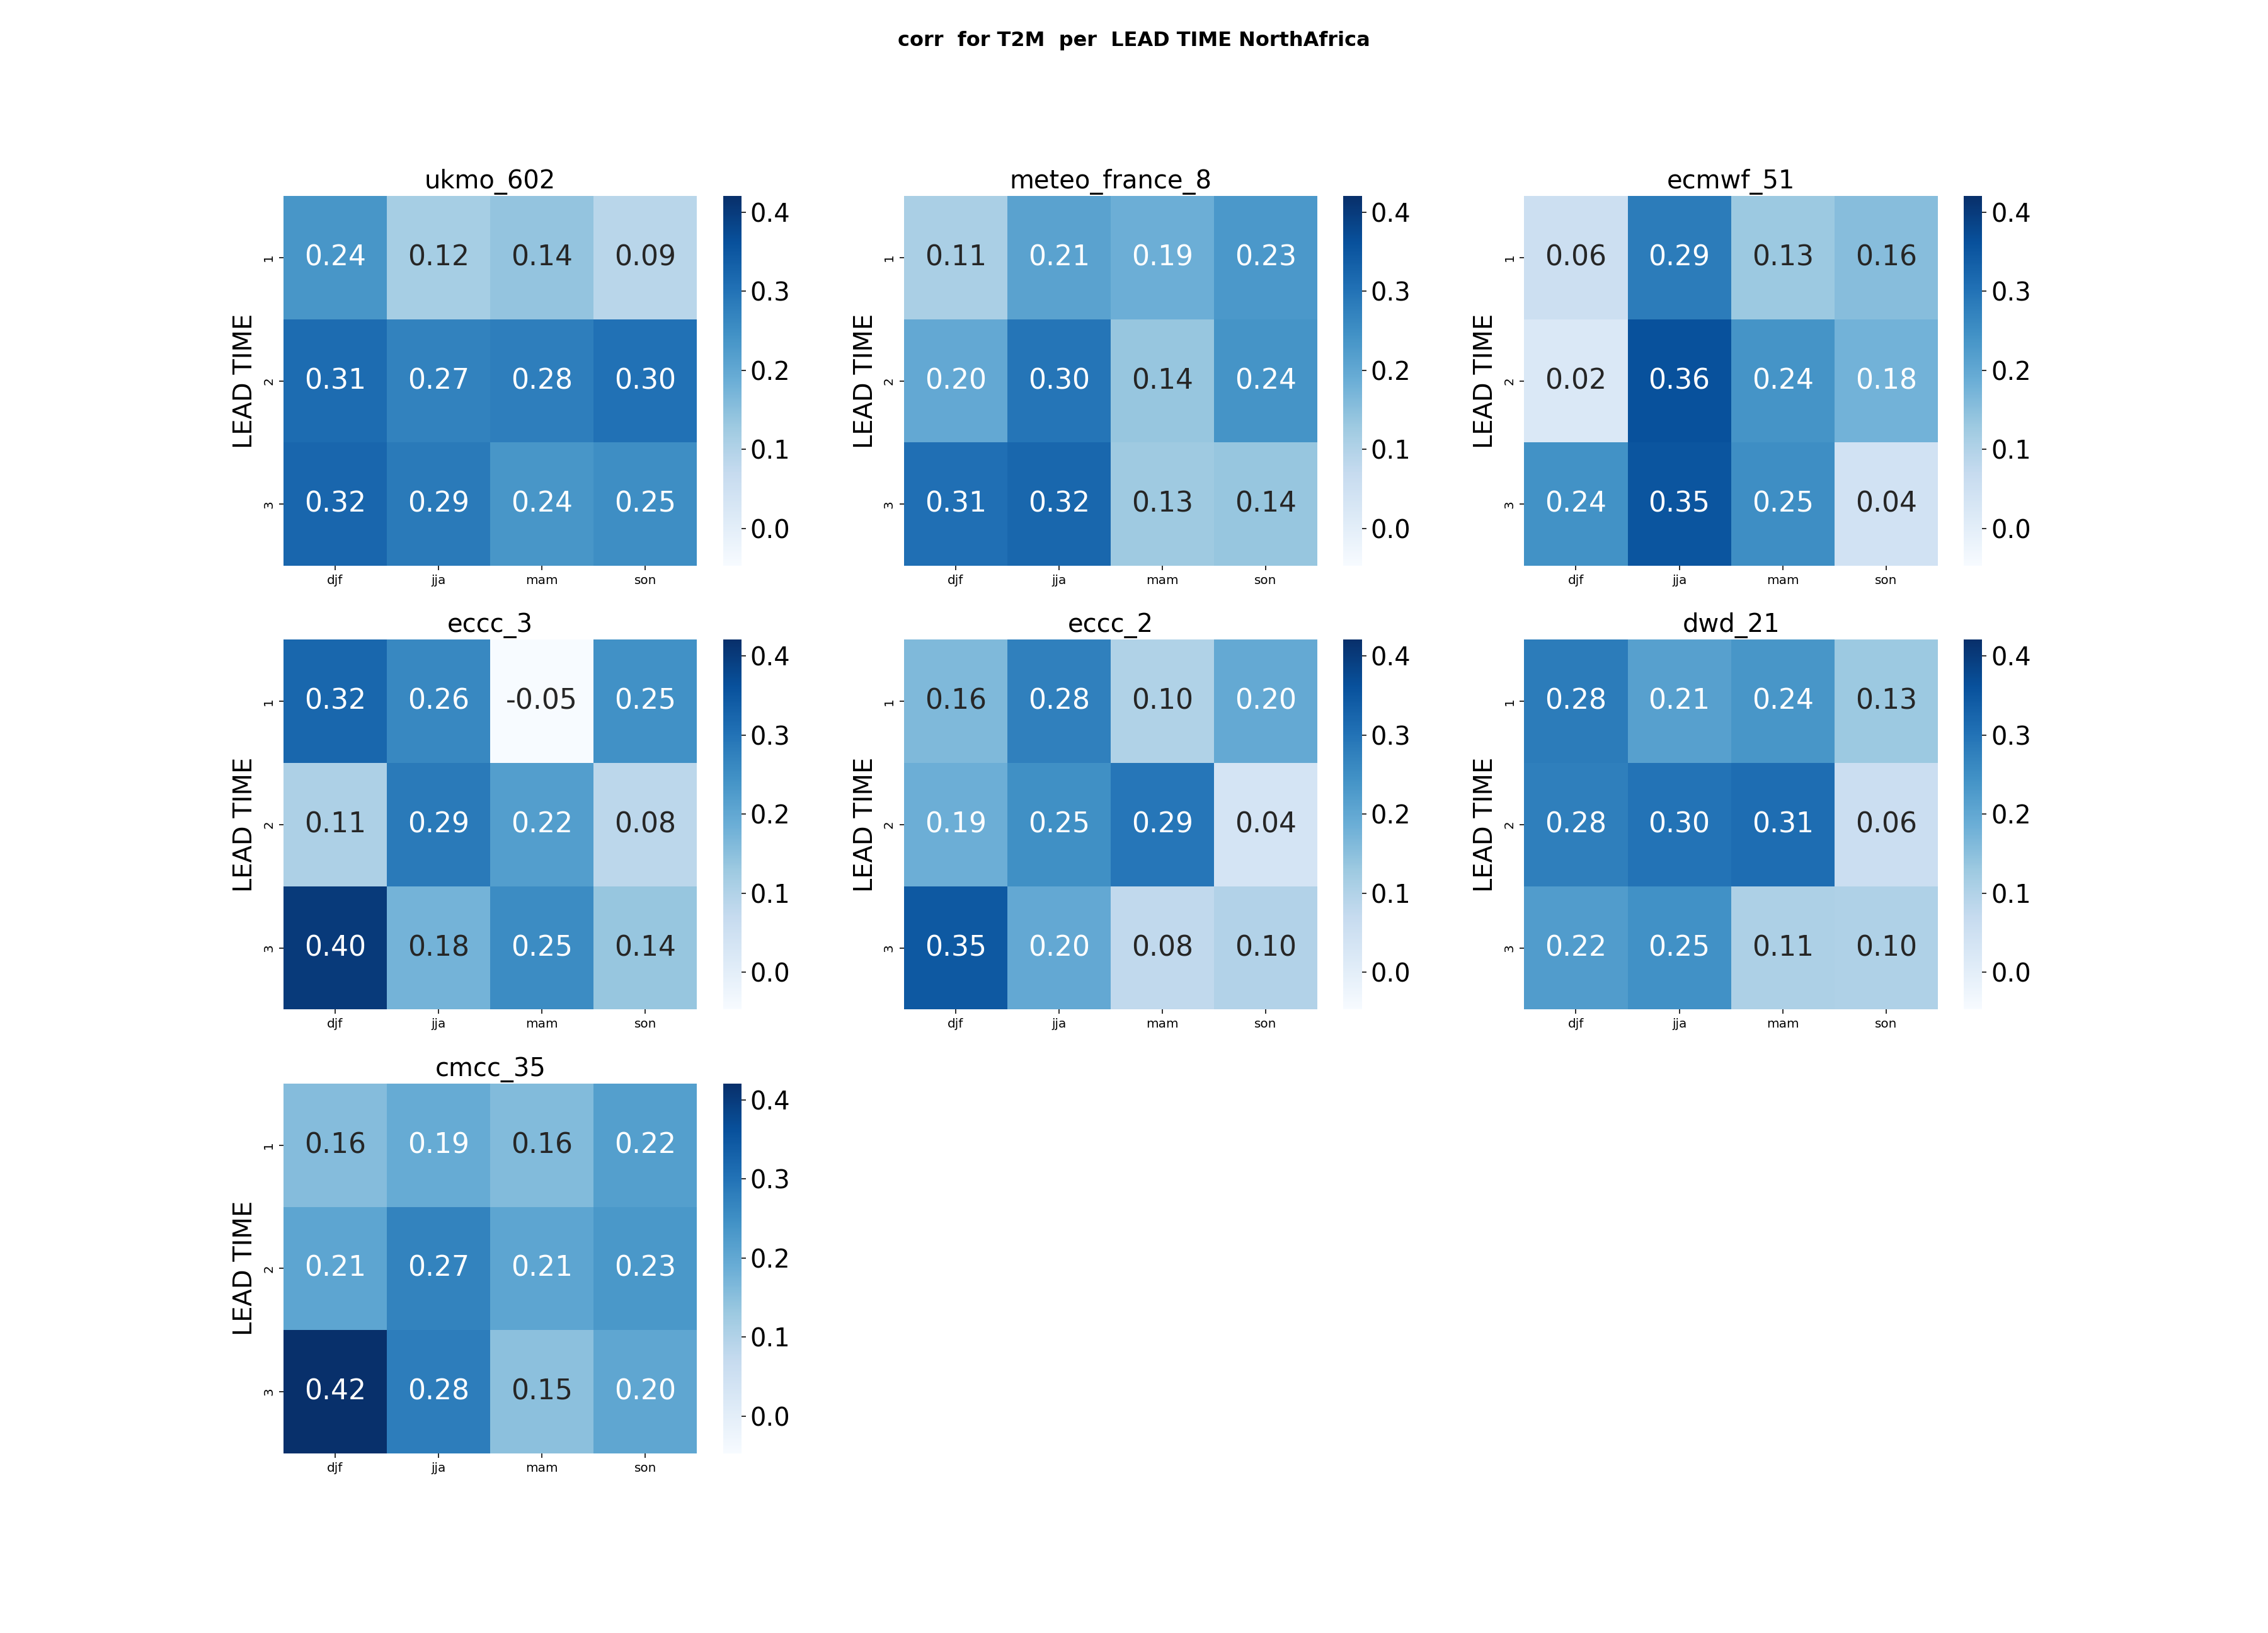
\includegraphics[width=1\linewidth]{plots/det/corr/corr_T2M_NorthAfrica.png}
    \caption{Temperature heatmap for north africa}
   
    \label{CORR_mam_t2m.png}
\end{figure}
\subsubsection{Root Mean Square Error}



\begin{figure}[H]
    \centering
    \includegraphics[width=1\linewidth]{plots/det/rmse/rmse_T2M_NorthAfrica.png}
    \caption{Temperature heatmap for north africa}
   
    \label{CORR_mam_t2m.png}
\end{figure}


\subsubsection{coefficient of determination}




\begin{figure}[H]
    \centering
    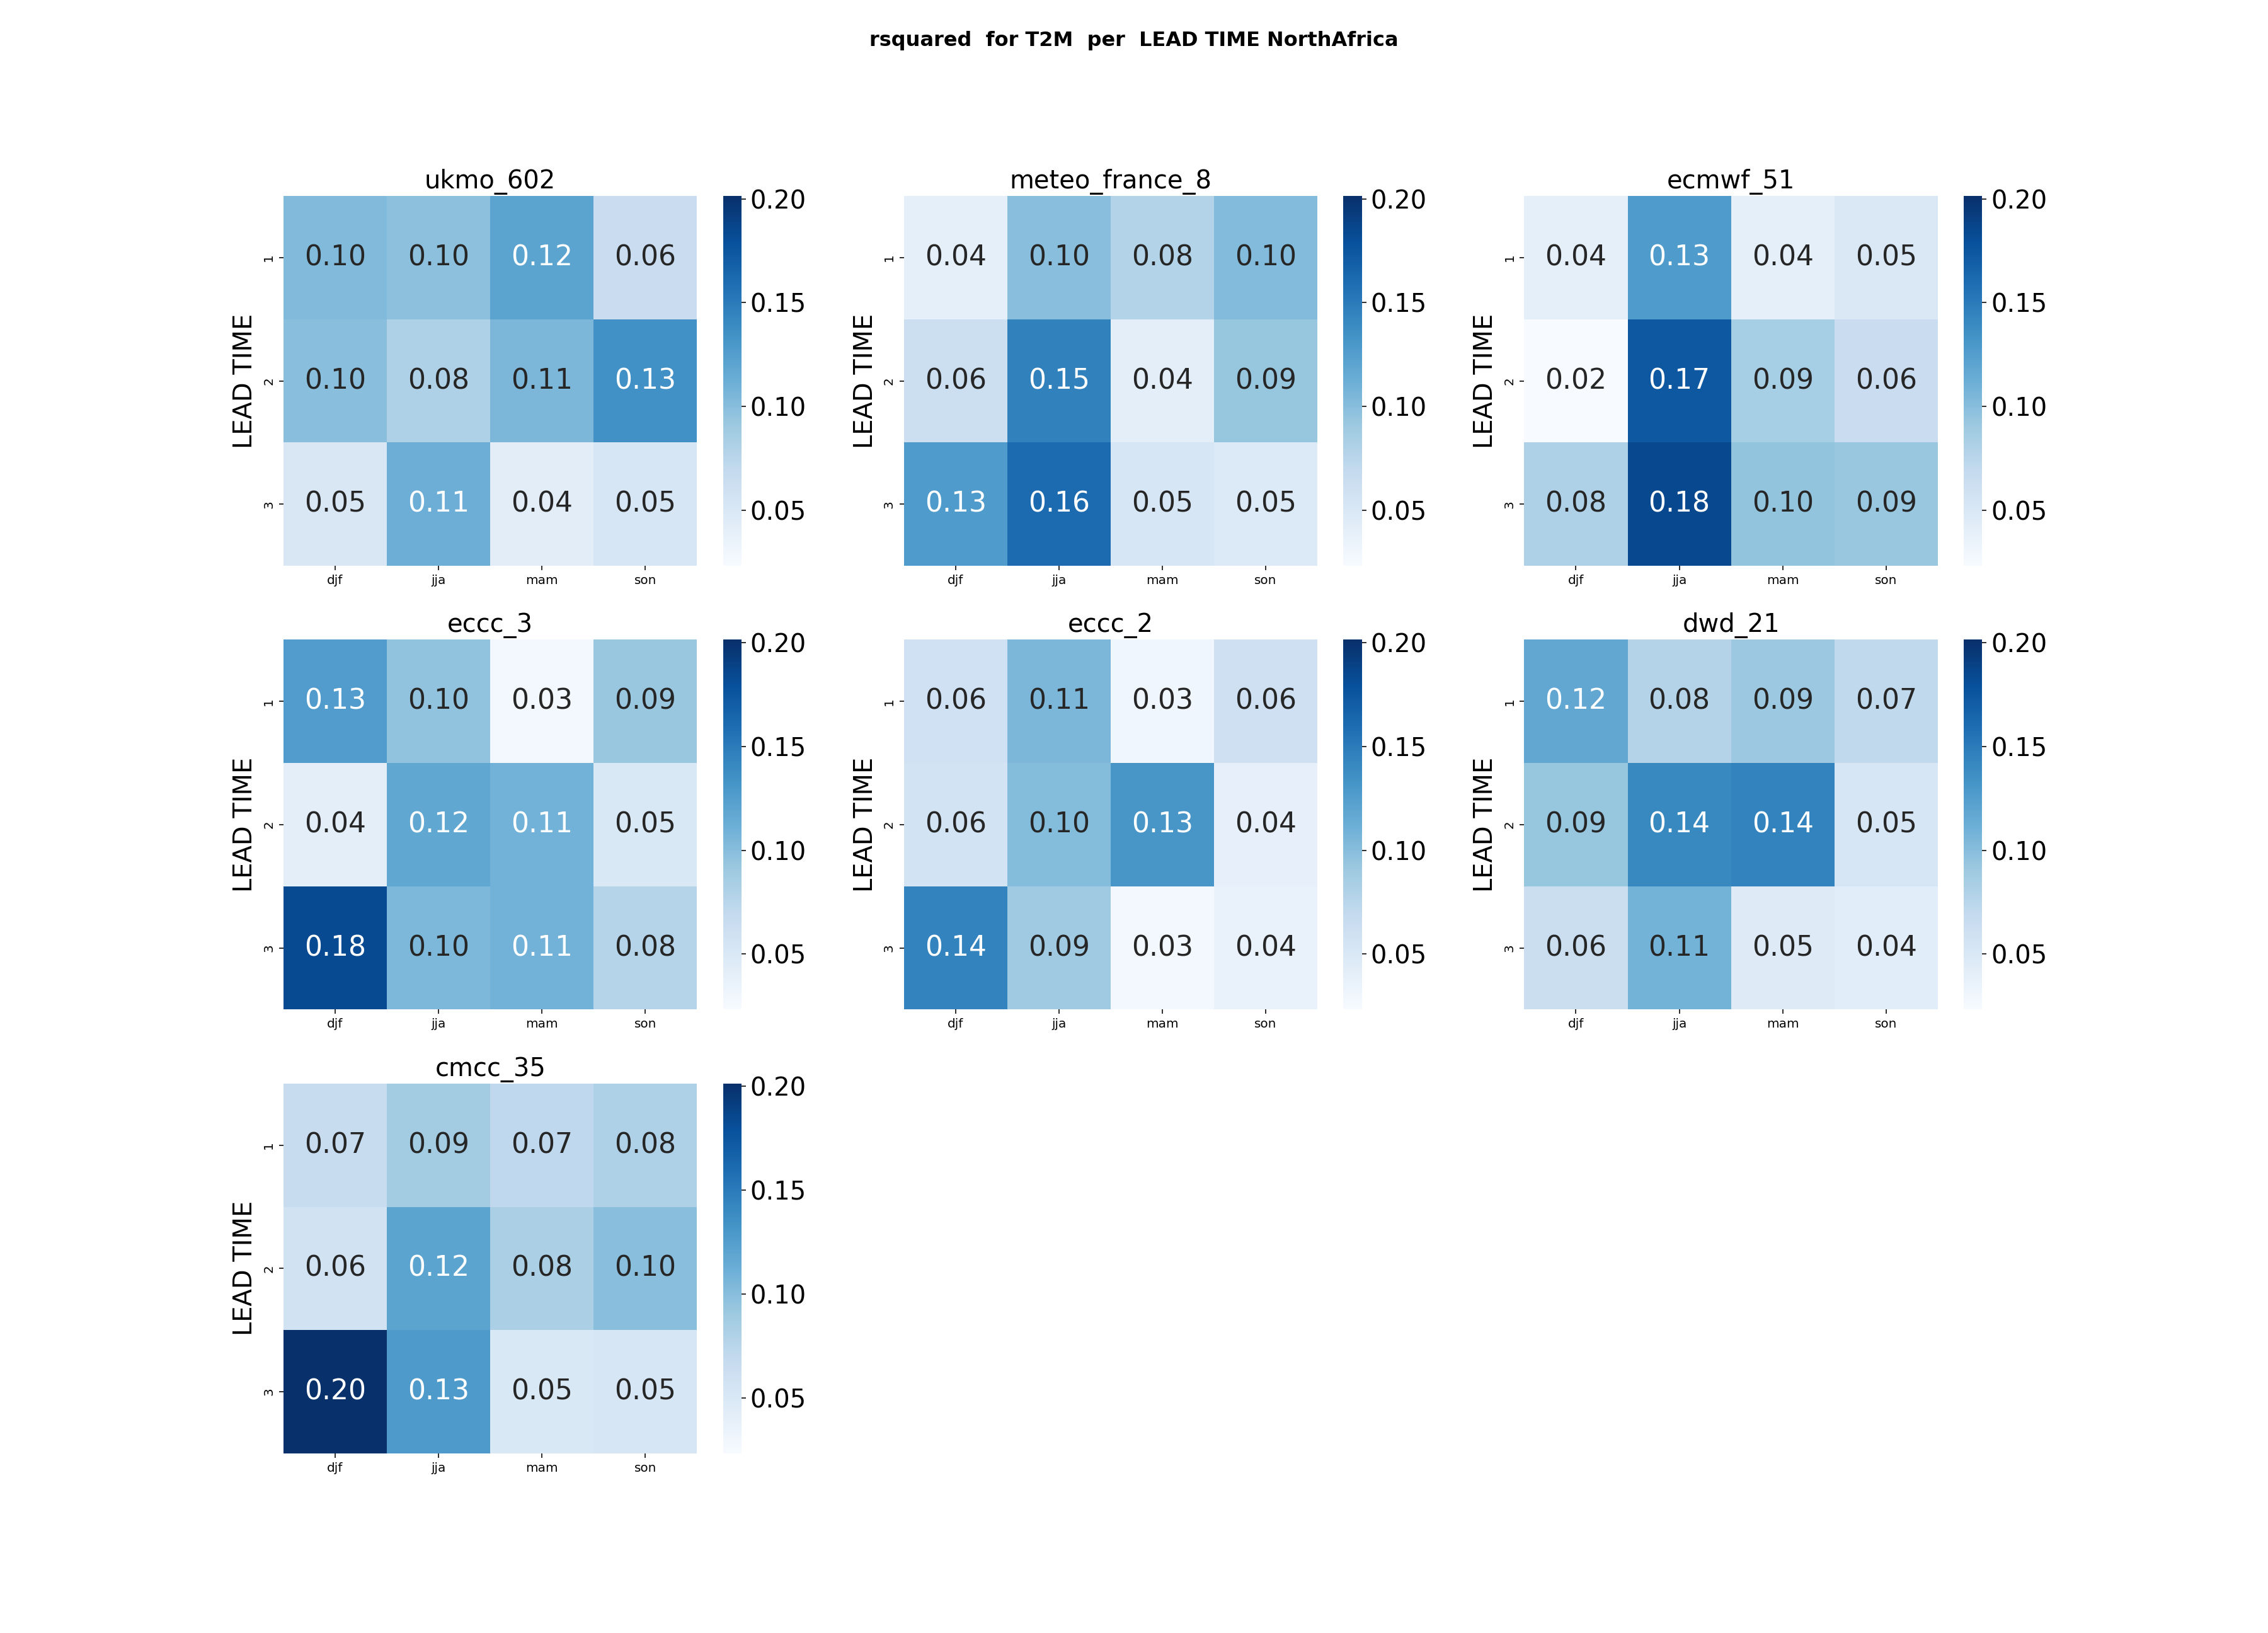
\includegraphics[width=1\linewidth]{plots/det/rsquared/rsquared_T2M_NorthAfrica.png}
    \caption{Temperature rsquared heatmaps for all the seasons for north africa}
    \label{fig:CORR_djf_t2m}
\end{figure}



\subsection{Probabilistic evaluation results}
\subsubsection{\textbf{Brier score}}


\begin{figure}[H]
    \centering
    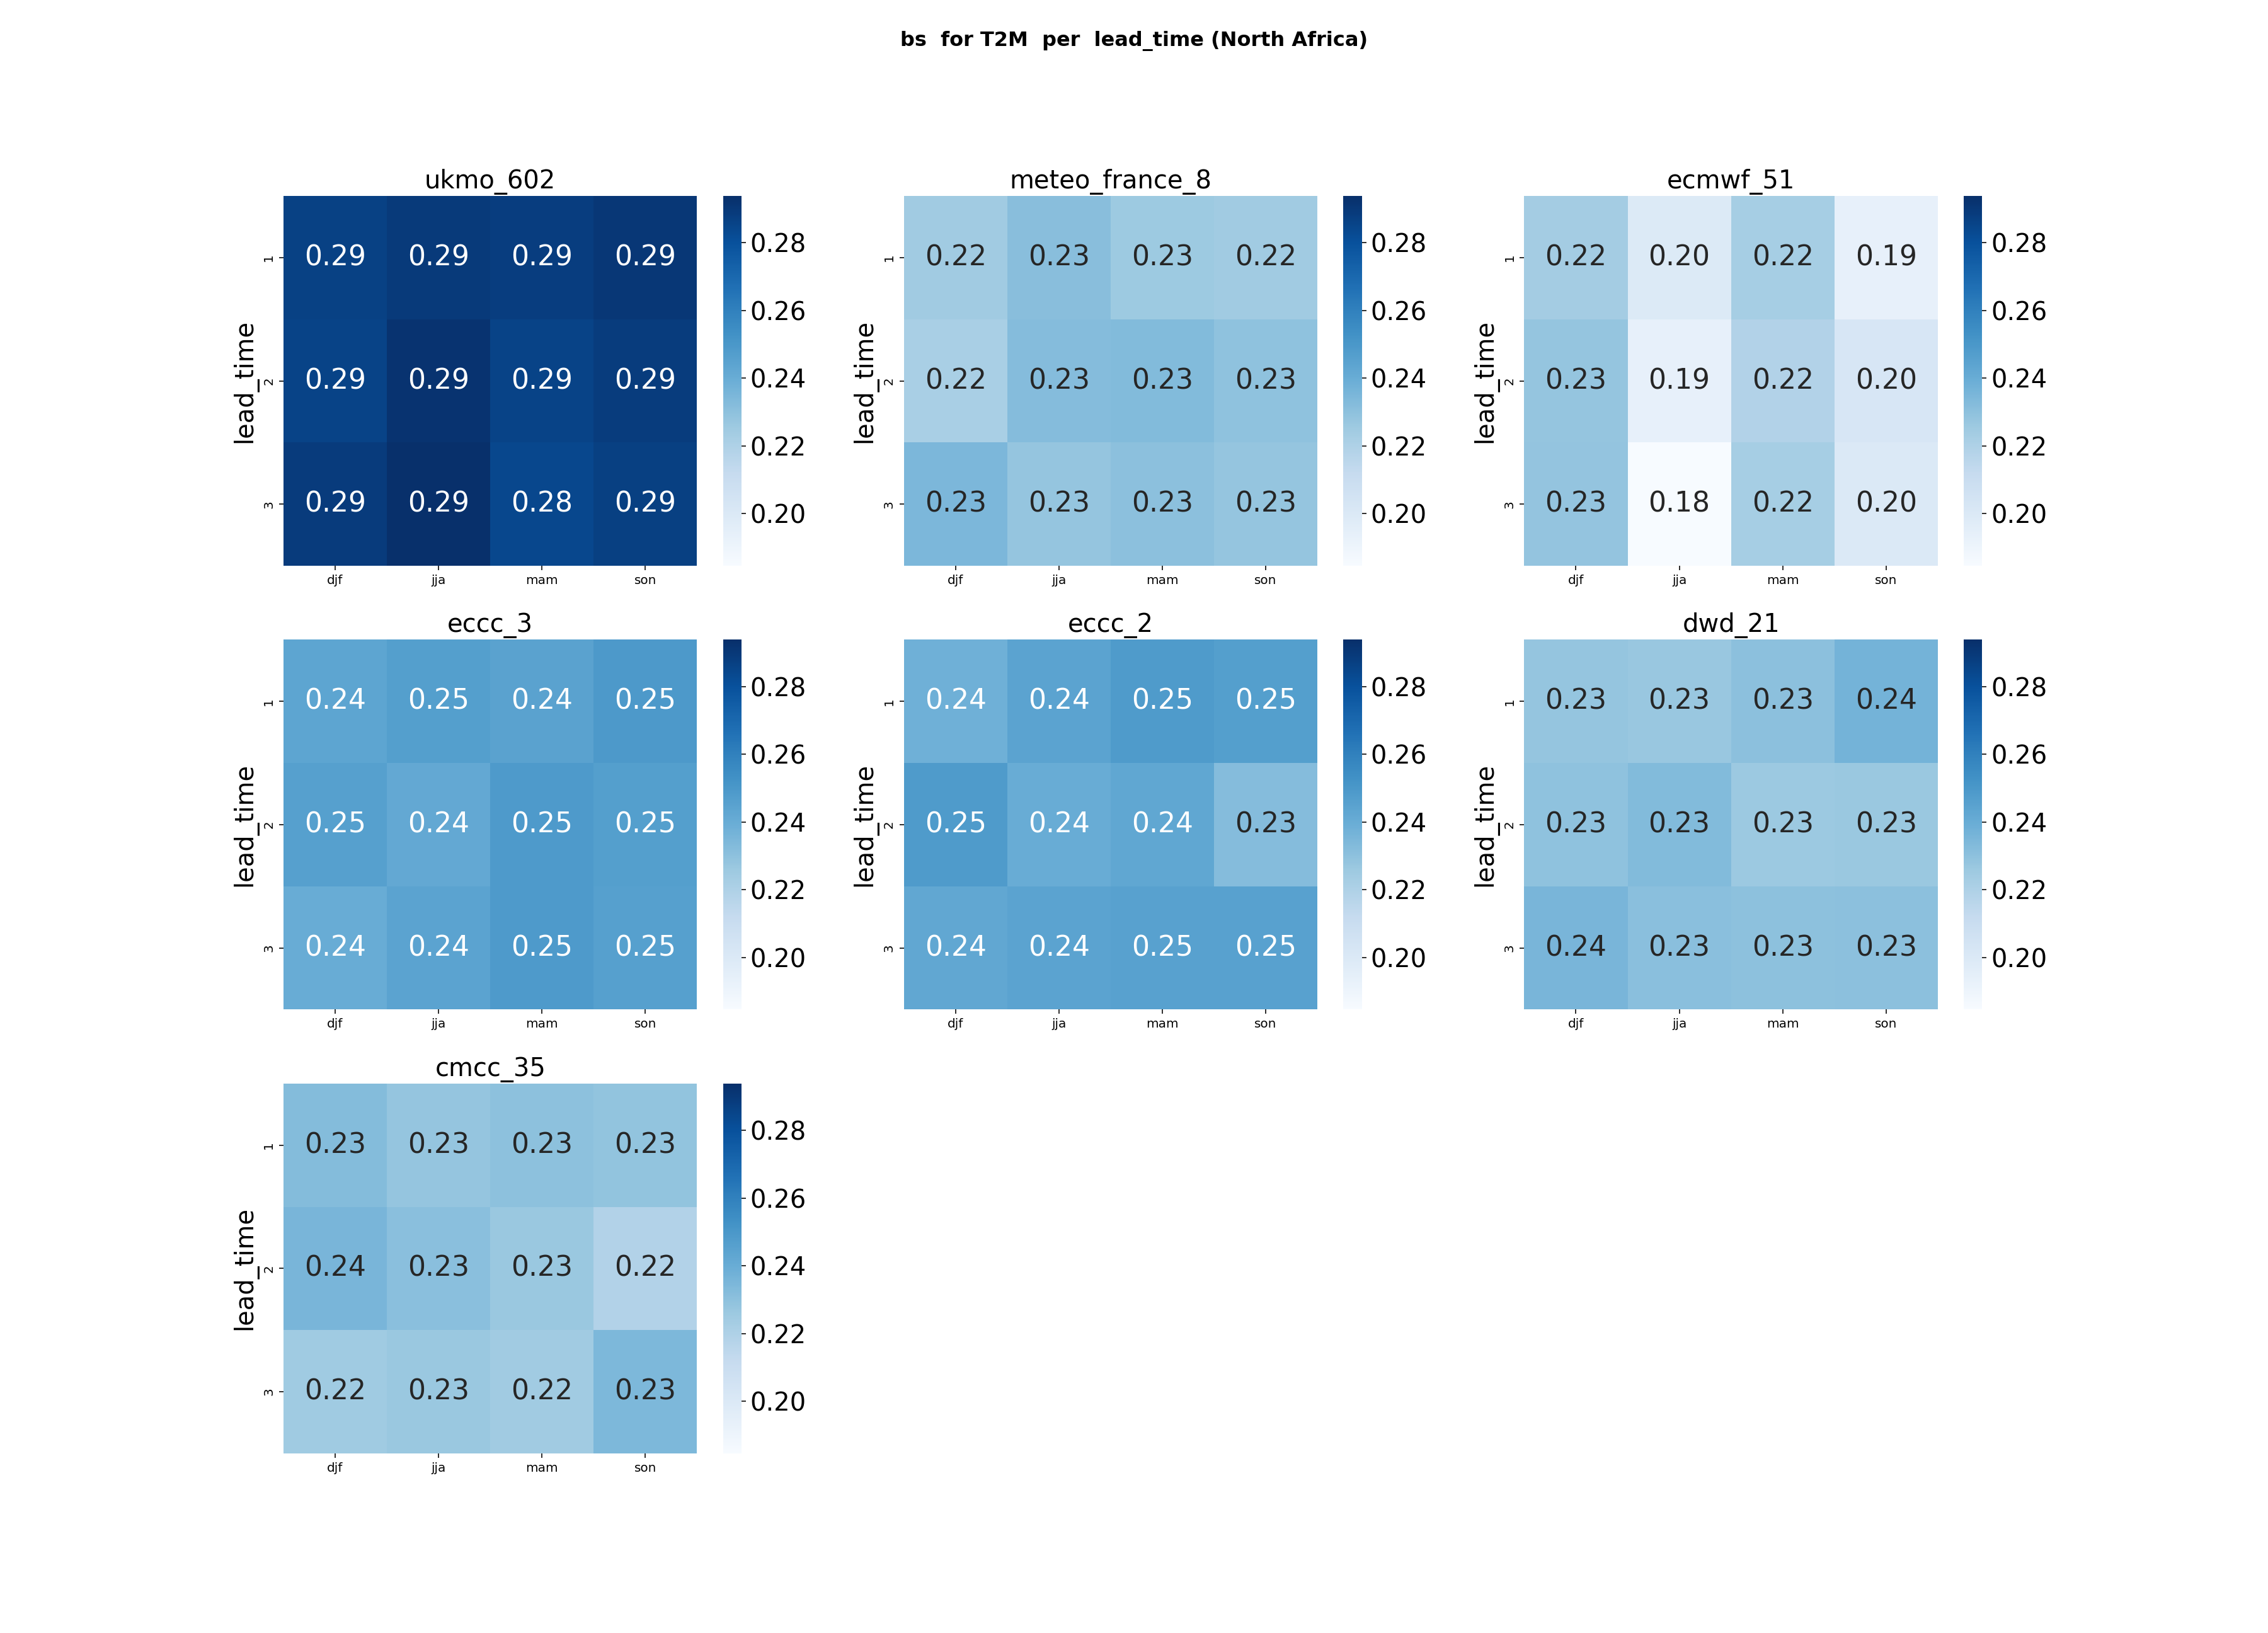
\includegraphics[width=1\linewidth]{plots/prob/bs/bs_T2M_lead_time_NorthAfrica.png}
    \caption{Temperature brier score heatmaps for all the seasons per lead time}
    \label{fig:CORR_djf_t2m}
\end{figure}

\subsubsection{\textbf{Reliability}}

\begin{figure}[H]
    \centering
    \includegraphics[width=1\linewidth]{plots/prob/rela/rela_T2M_NorthAfrica.png}
    \caption{temperature reliabilty heatmap for north africa}
    \label{CORR_mam_t2m.png}
\end{figure}





\subsubsection{\textbf{The ranked probability score }}



\begin{figure}[H]
    \centering
    \includegraphics[width=1\linewidth]{plots/prob/rps/rps_T2M_NorthAfrica.png}
    \caption{Temperature RPS  heatmaps for north africa}
    \label{fig:CORR_djf_t2m}
\end{figure}
\subsubsection{Receiver Operating Characteristic}

\begin{figure}[H]
    \centering
    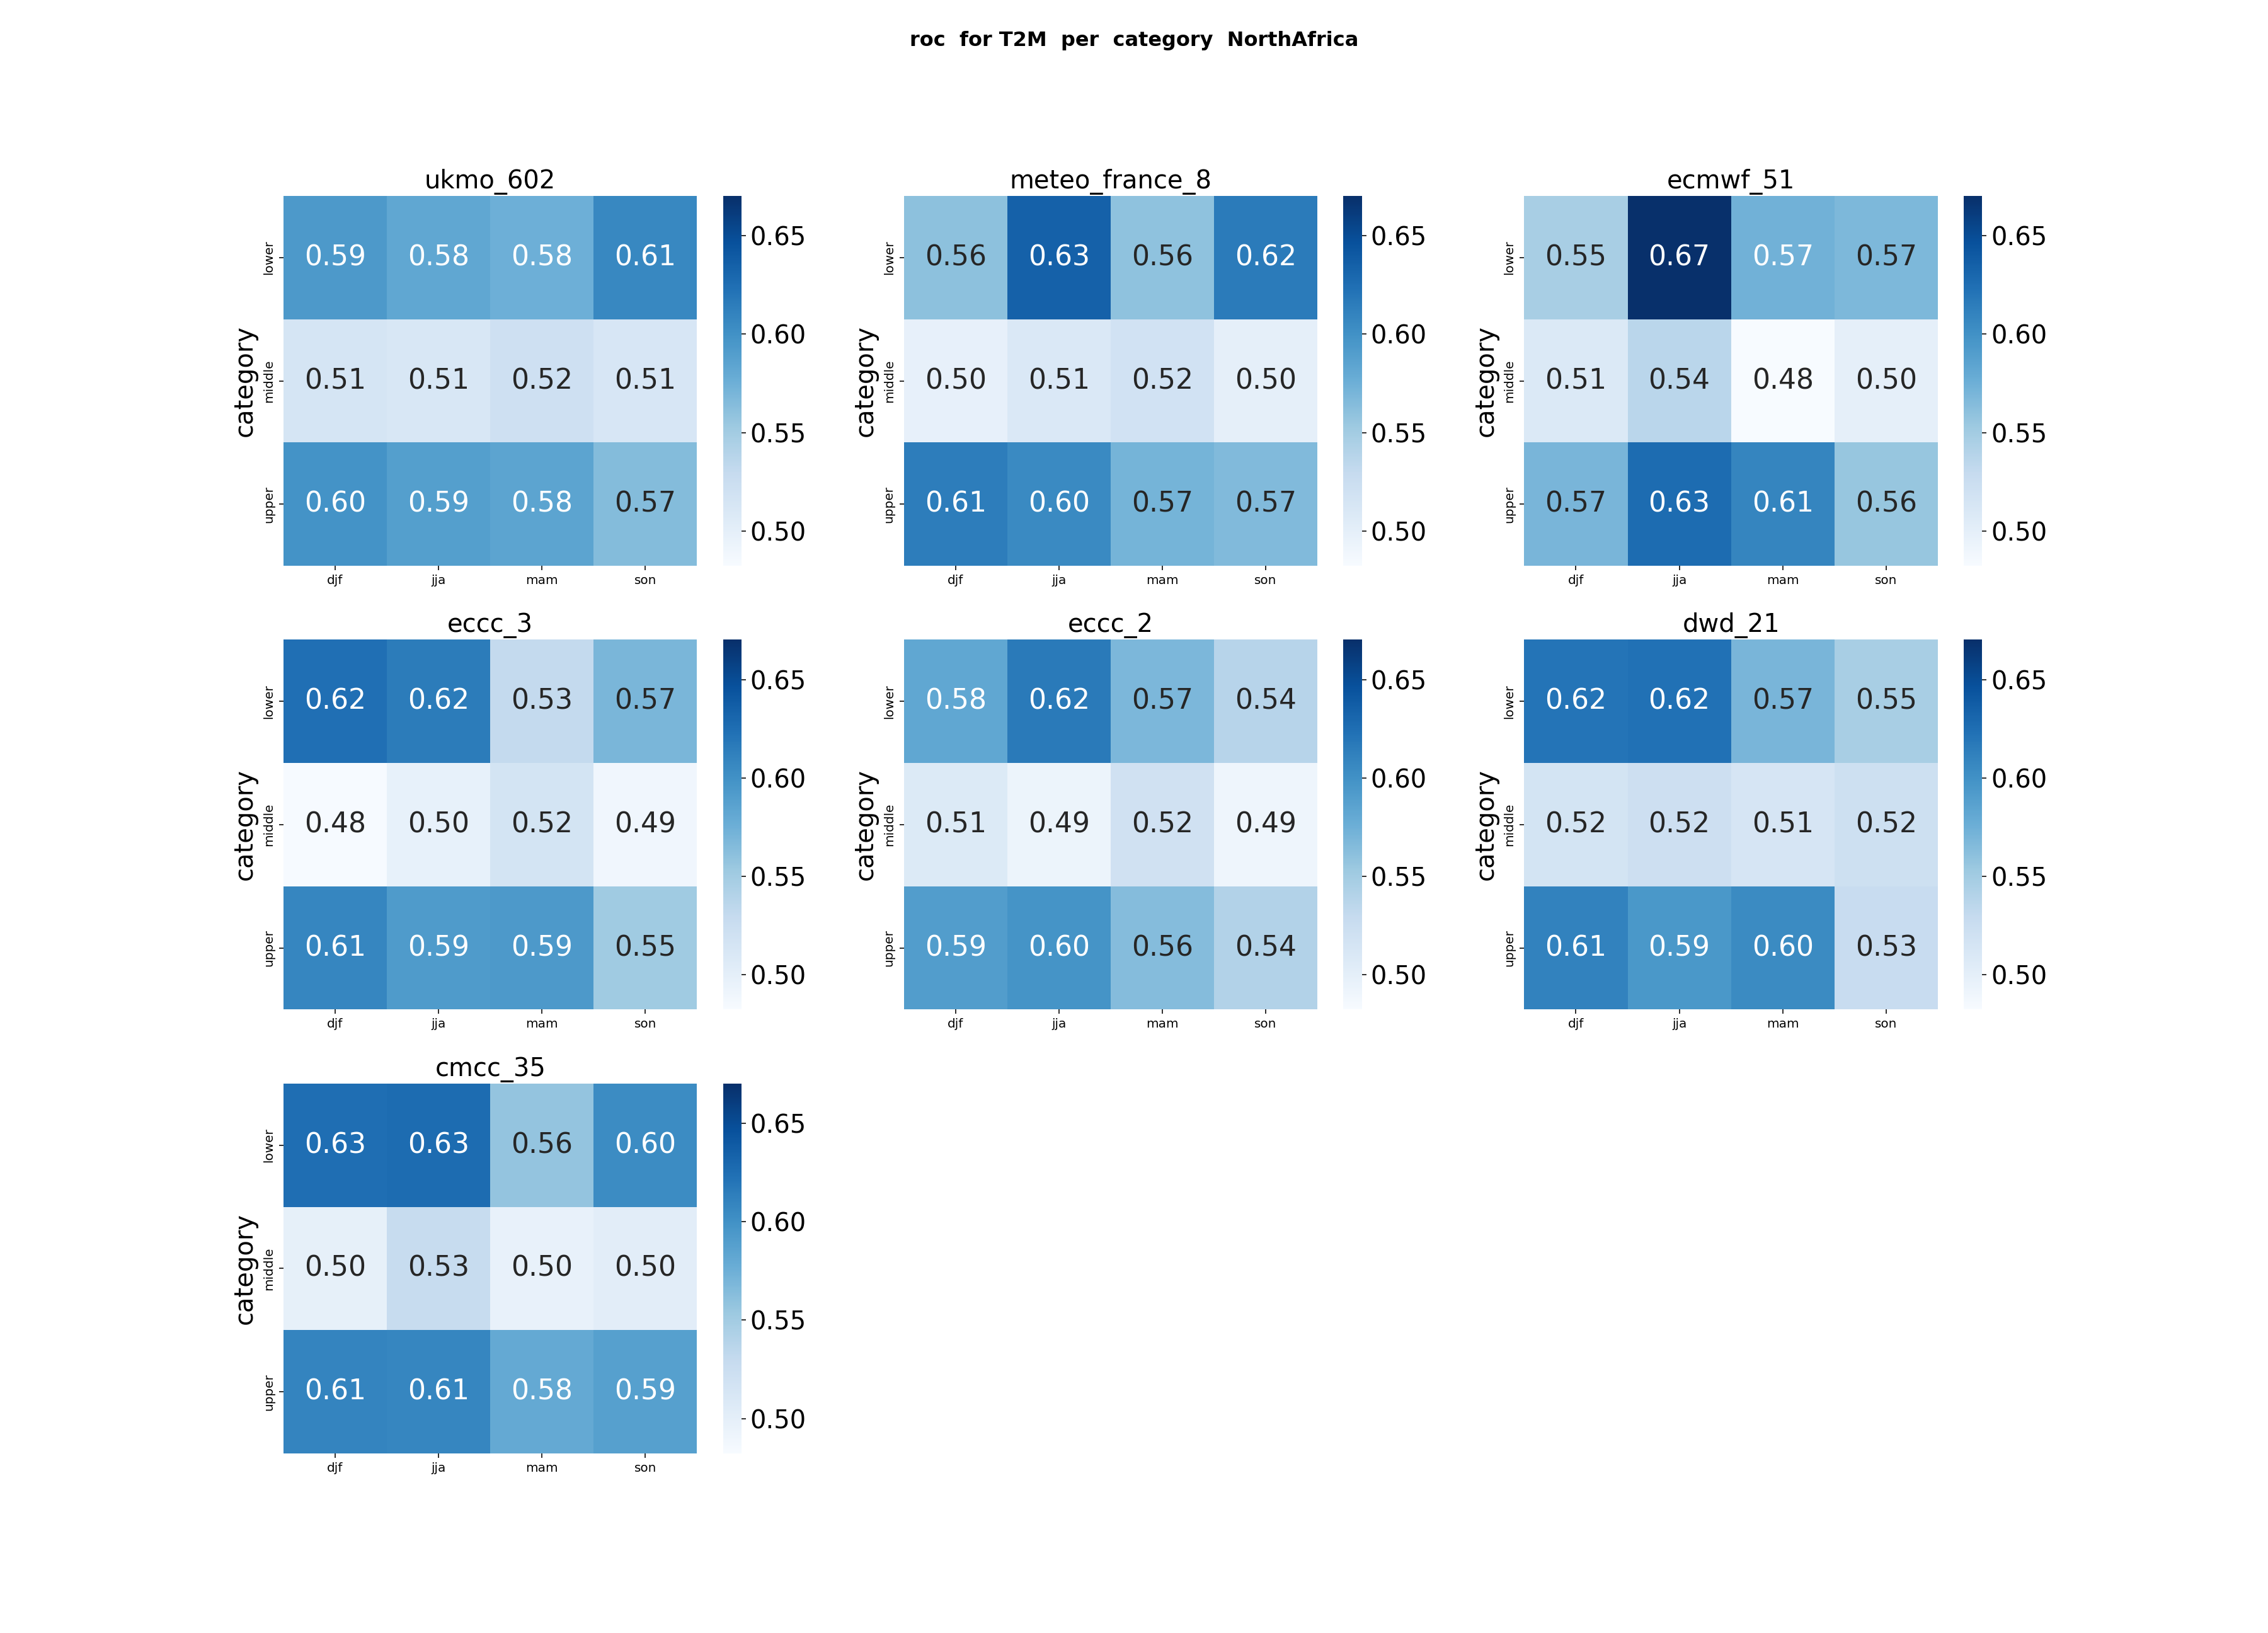
\includegraphics[width=1\linewidth]{plots/prob/roc/roc_T2M_category_NorthAfrica.png}
    \caption{Temperature AUC  heatmaps for north africa }
    \label{fig:CORR_djf_t2m}
\end{figure}


\subsubsection{Relative operating characteristics Skill Score}


\begin{figure}[H]
    \centering
    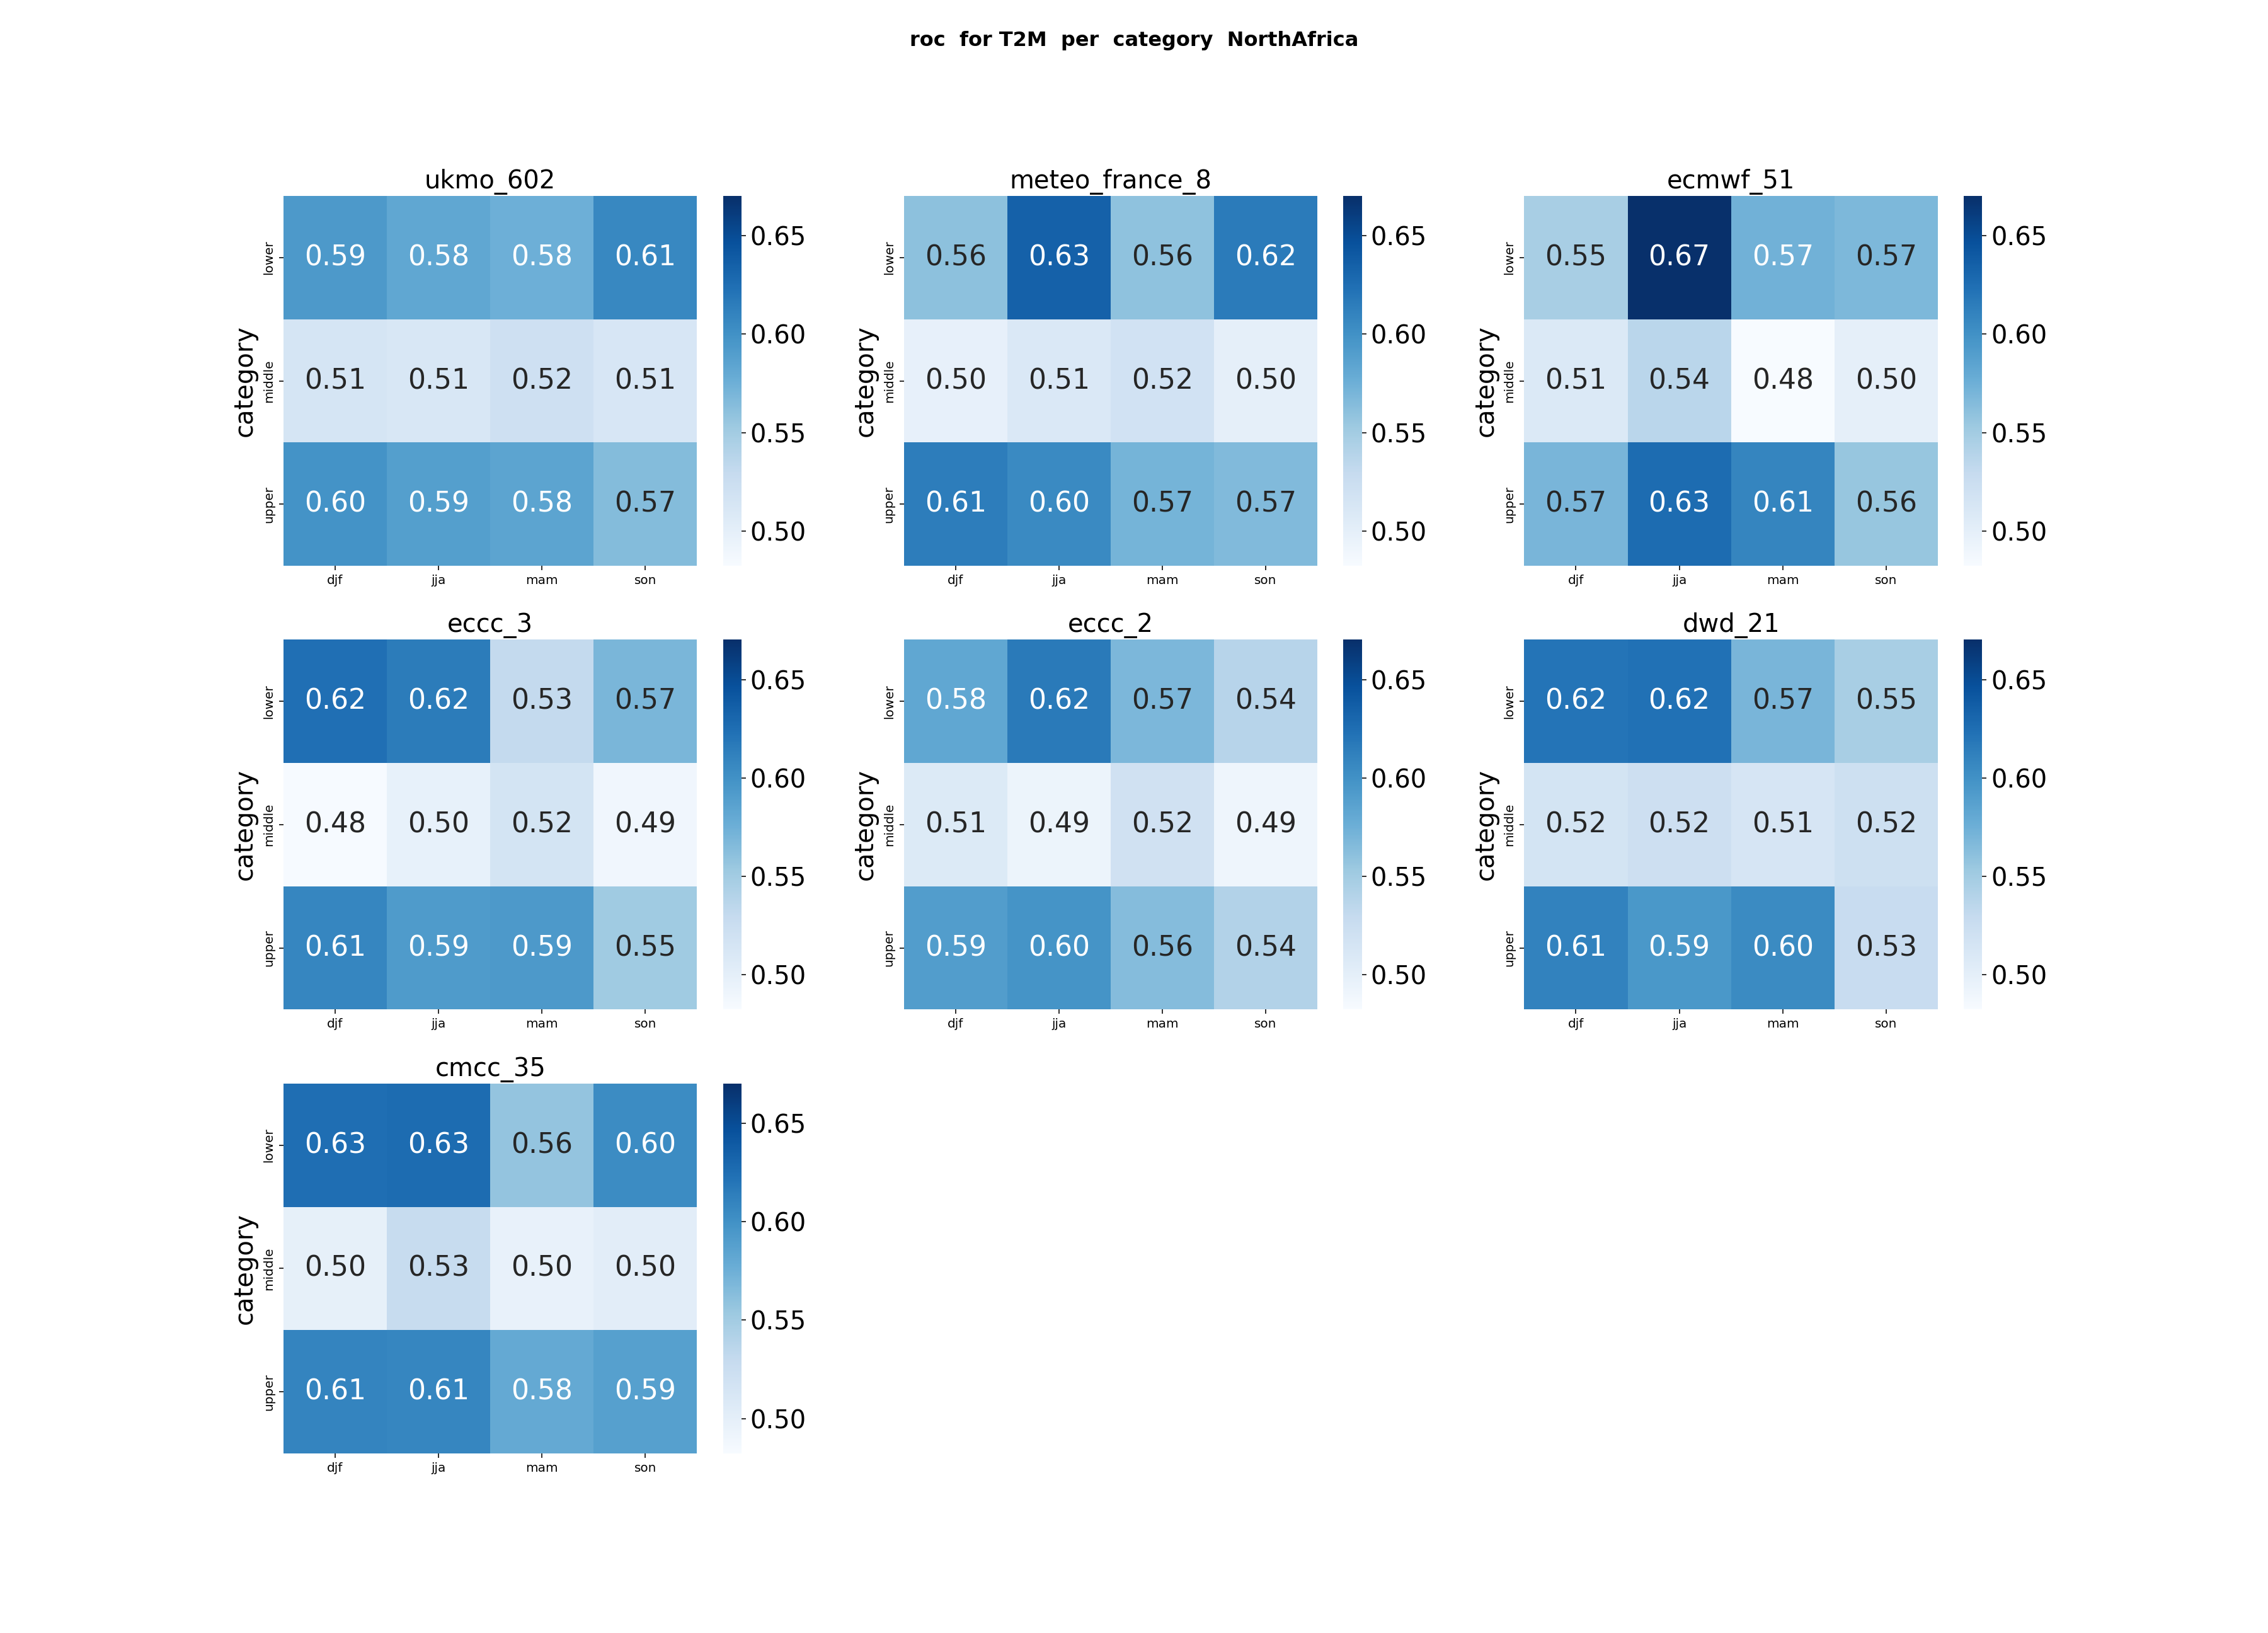
\includegraphics[width=1\linewidth]{plots/prob/roc/roc_T2M_category_NorthAfrica.png}
    \caption{Temperature ROCSS  heatmaps for north africa }
    \label{fig:CORR_djf_t2m}
\end{figure}





















\section{PRECIPITATIONS}
\subsection{Deterministic Evaluation Metrics}


\subsubsection{Spearman rank correlation}



\begin{figure}[H]
	\centering
	\includegraphics[scale=0.25]{plots/det/corr/corr_RR_NorthAfrica.png}
	\caption{The Heatmap of correlation for the north africa region for every period \textbf{\textit{(1 for perfect Correlation)} }}
\end{figure}
In general, the performance is in the same scale as the MENA region. The \textbf{\textit{ecmwf,ukmo and meteo-france}} show moderate correlation, especially for the first lead-time. The correlation for the third lead-time isn't so good, except for the cmcc_35 that shows better results. As well as the previous analysis, in the MENA region, the SON knows an unusual good performance in the second lead-time.


\subsubsection{RMSE}
 

\begin{figure}[H]
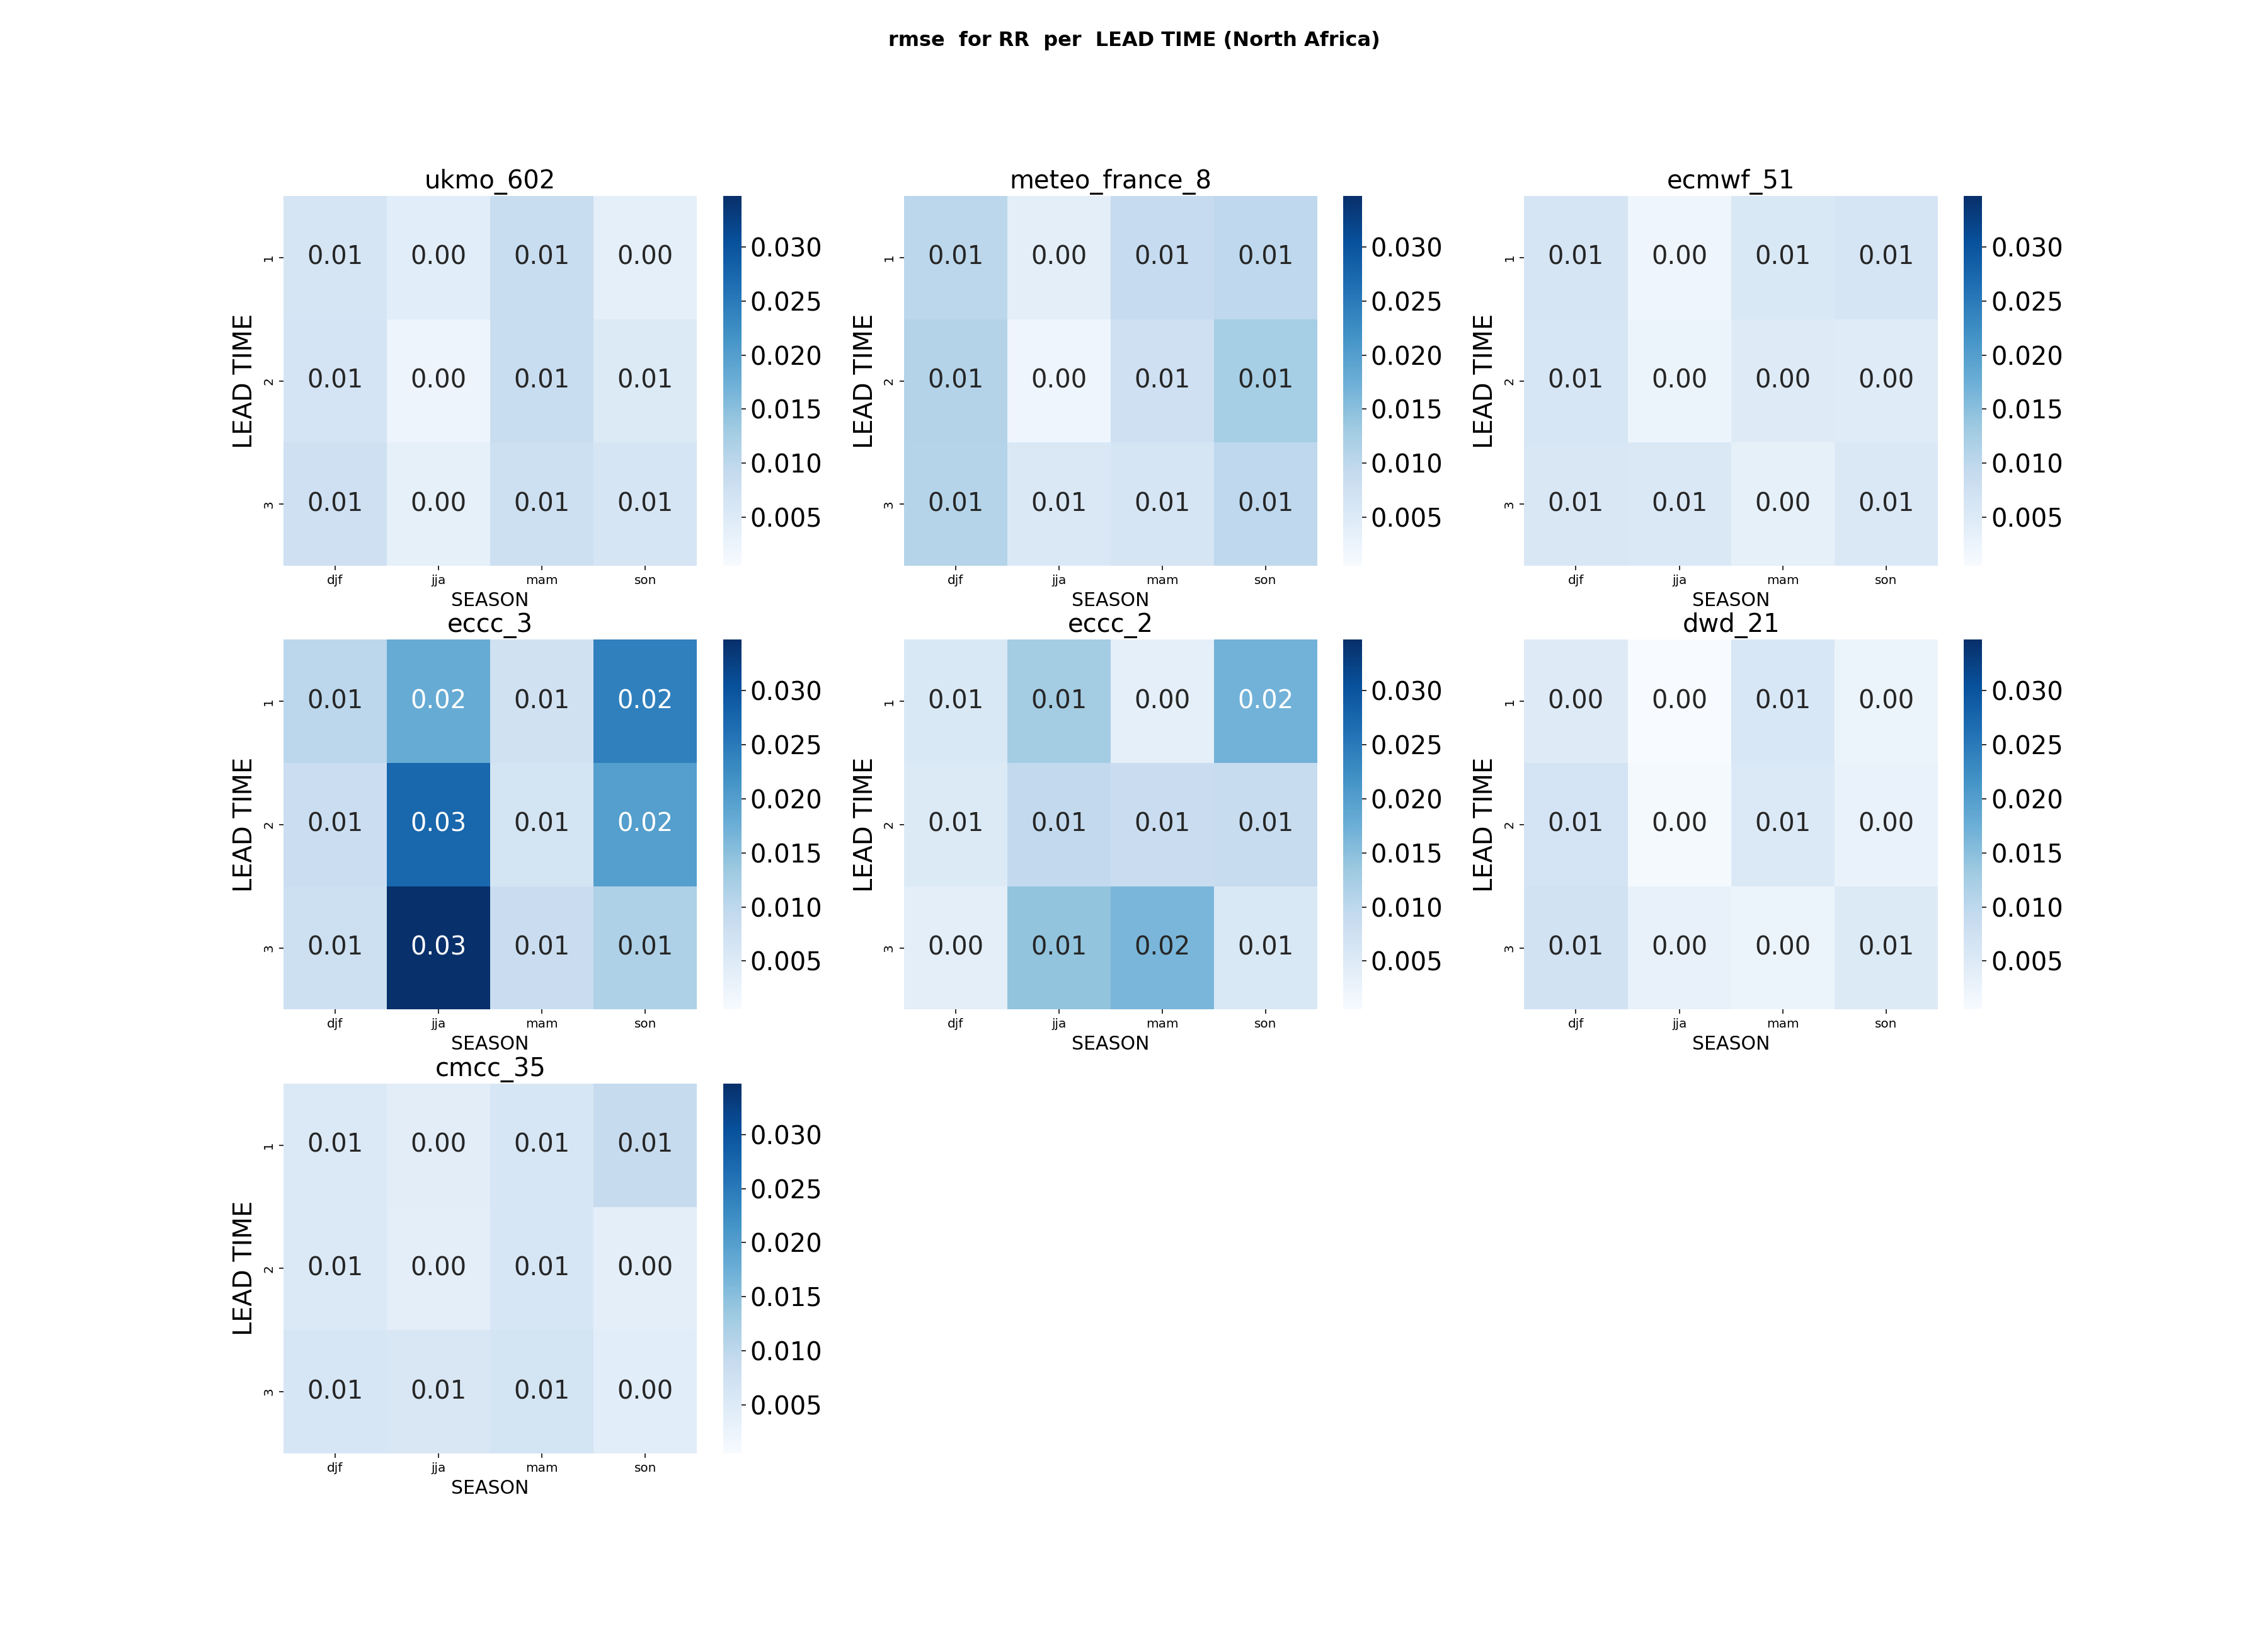
\includegraphics[scale=0.3]{plots/det/rmse/rmse_RR_NorthAfrica.png}
\caption{The Heatmap of RMSE for Precipitations in the north africa region for every period}
\end{figure}

the RMSE, is better for the North Africa with relatively low values and good stability for all center and lead-times.

\subsubsection{Coefficient of Determination (\( R^2 \))}
\begin{figure}[H]
	\centering
	\includegraphics[scale=0.25]{plots/det/rsquared/rsquared_RR_NorthAfrica.png}
	\caption{The Heatmap of rsquared for Precipitations in the north africa region for every period \textbf{\textit{(1 for perfect RSQUARED)} }}
\end{figure}

The R-SQUARED shows similar performance in North Africa, the values are very low for all centers and lead-times.


\subsection{Probabilistic Evaluation Metrics}

\subsubsection{The Brier Score (BS)}

\begin{figure}[H]
    \centering
    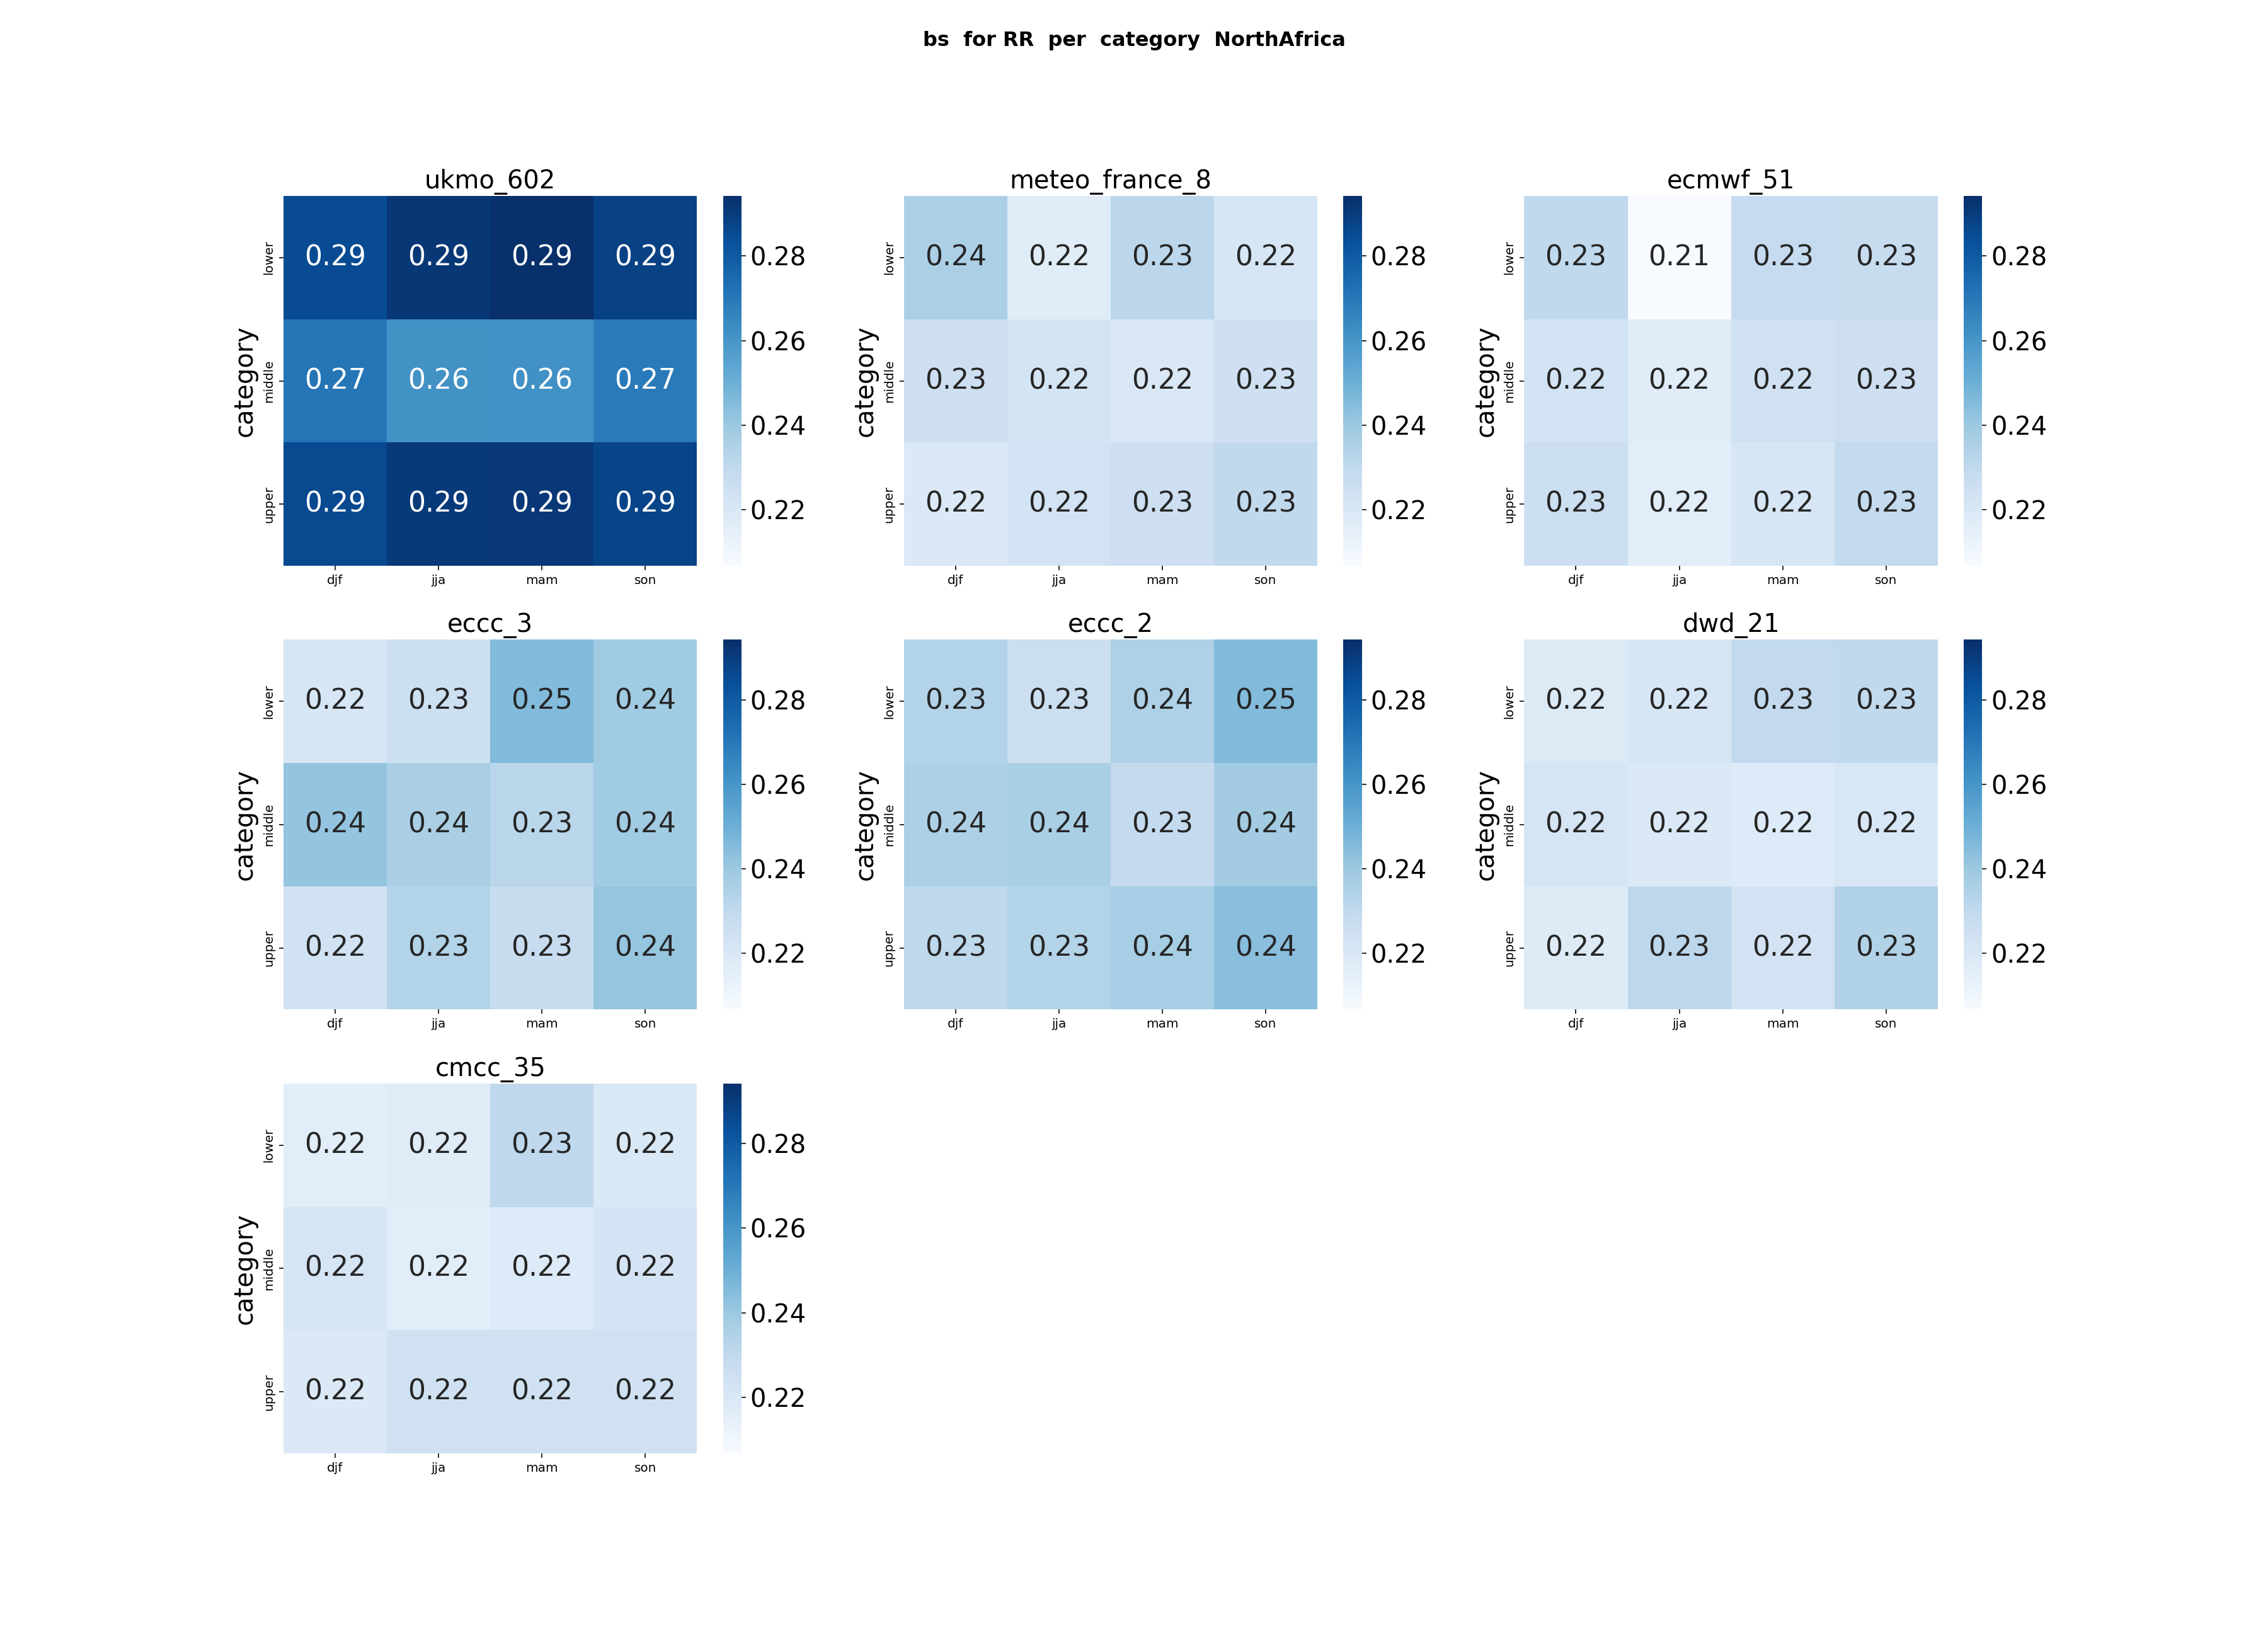
\includegraphics[scale=0.25]{plots/prob/bs/bs_RR_category_NorthAfrica.png}
    \caption{The Heatmap of Brier Score for each category  . \textbf{\textit{(0 represents perfect BS)}}}
\end{figure}


\begin{figure}[H]
    \centering
    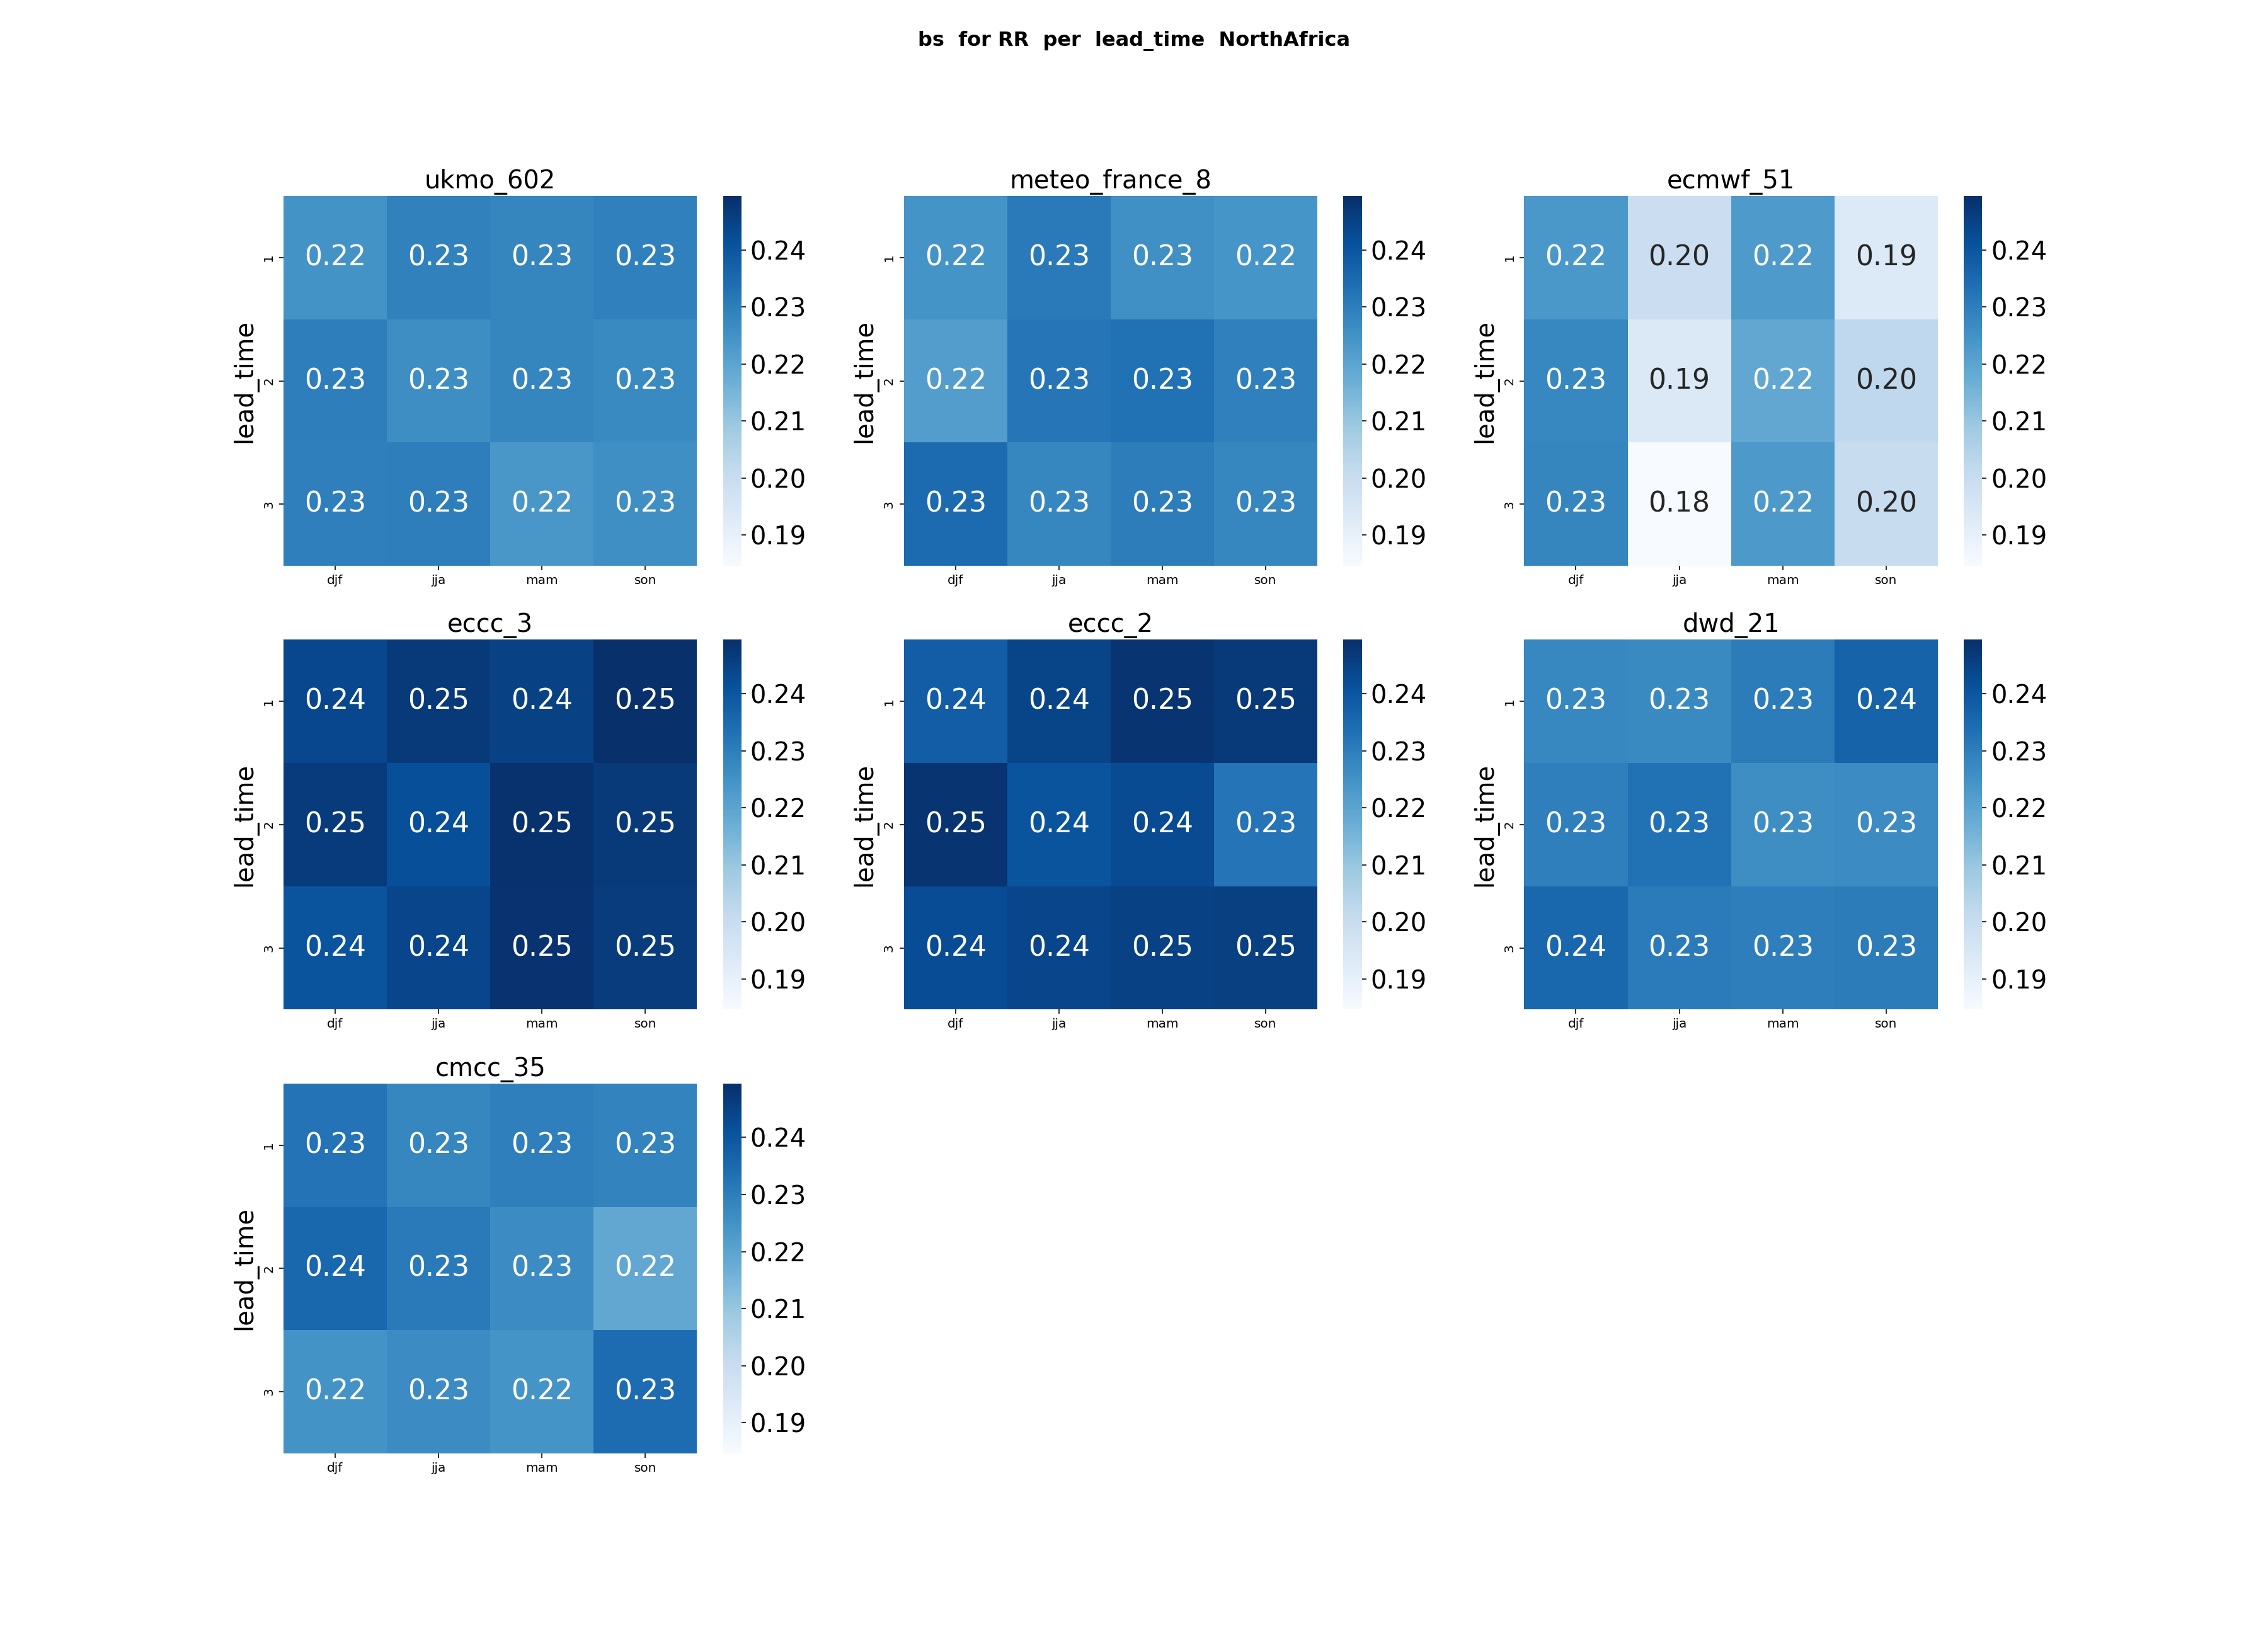
\includegraphics[scale=0.25]{plots/prob/bs/bs_RR_lead_time_NorthAfrica.png}
    \caption{The Heatmap of Brier Score for lead-time. \textbf{\textit{(0 represents perfect BS)}}}
\end{figure}

there is no big differences in term of Brier Score for North Africa, the scores are the same for both lead-times ad categories




\subsubsection{Reliability}

\begin{figure}[H]
    \centering
    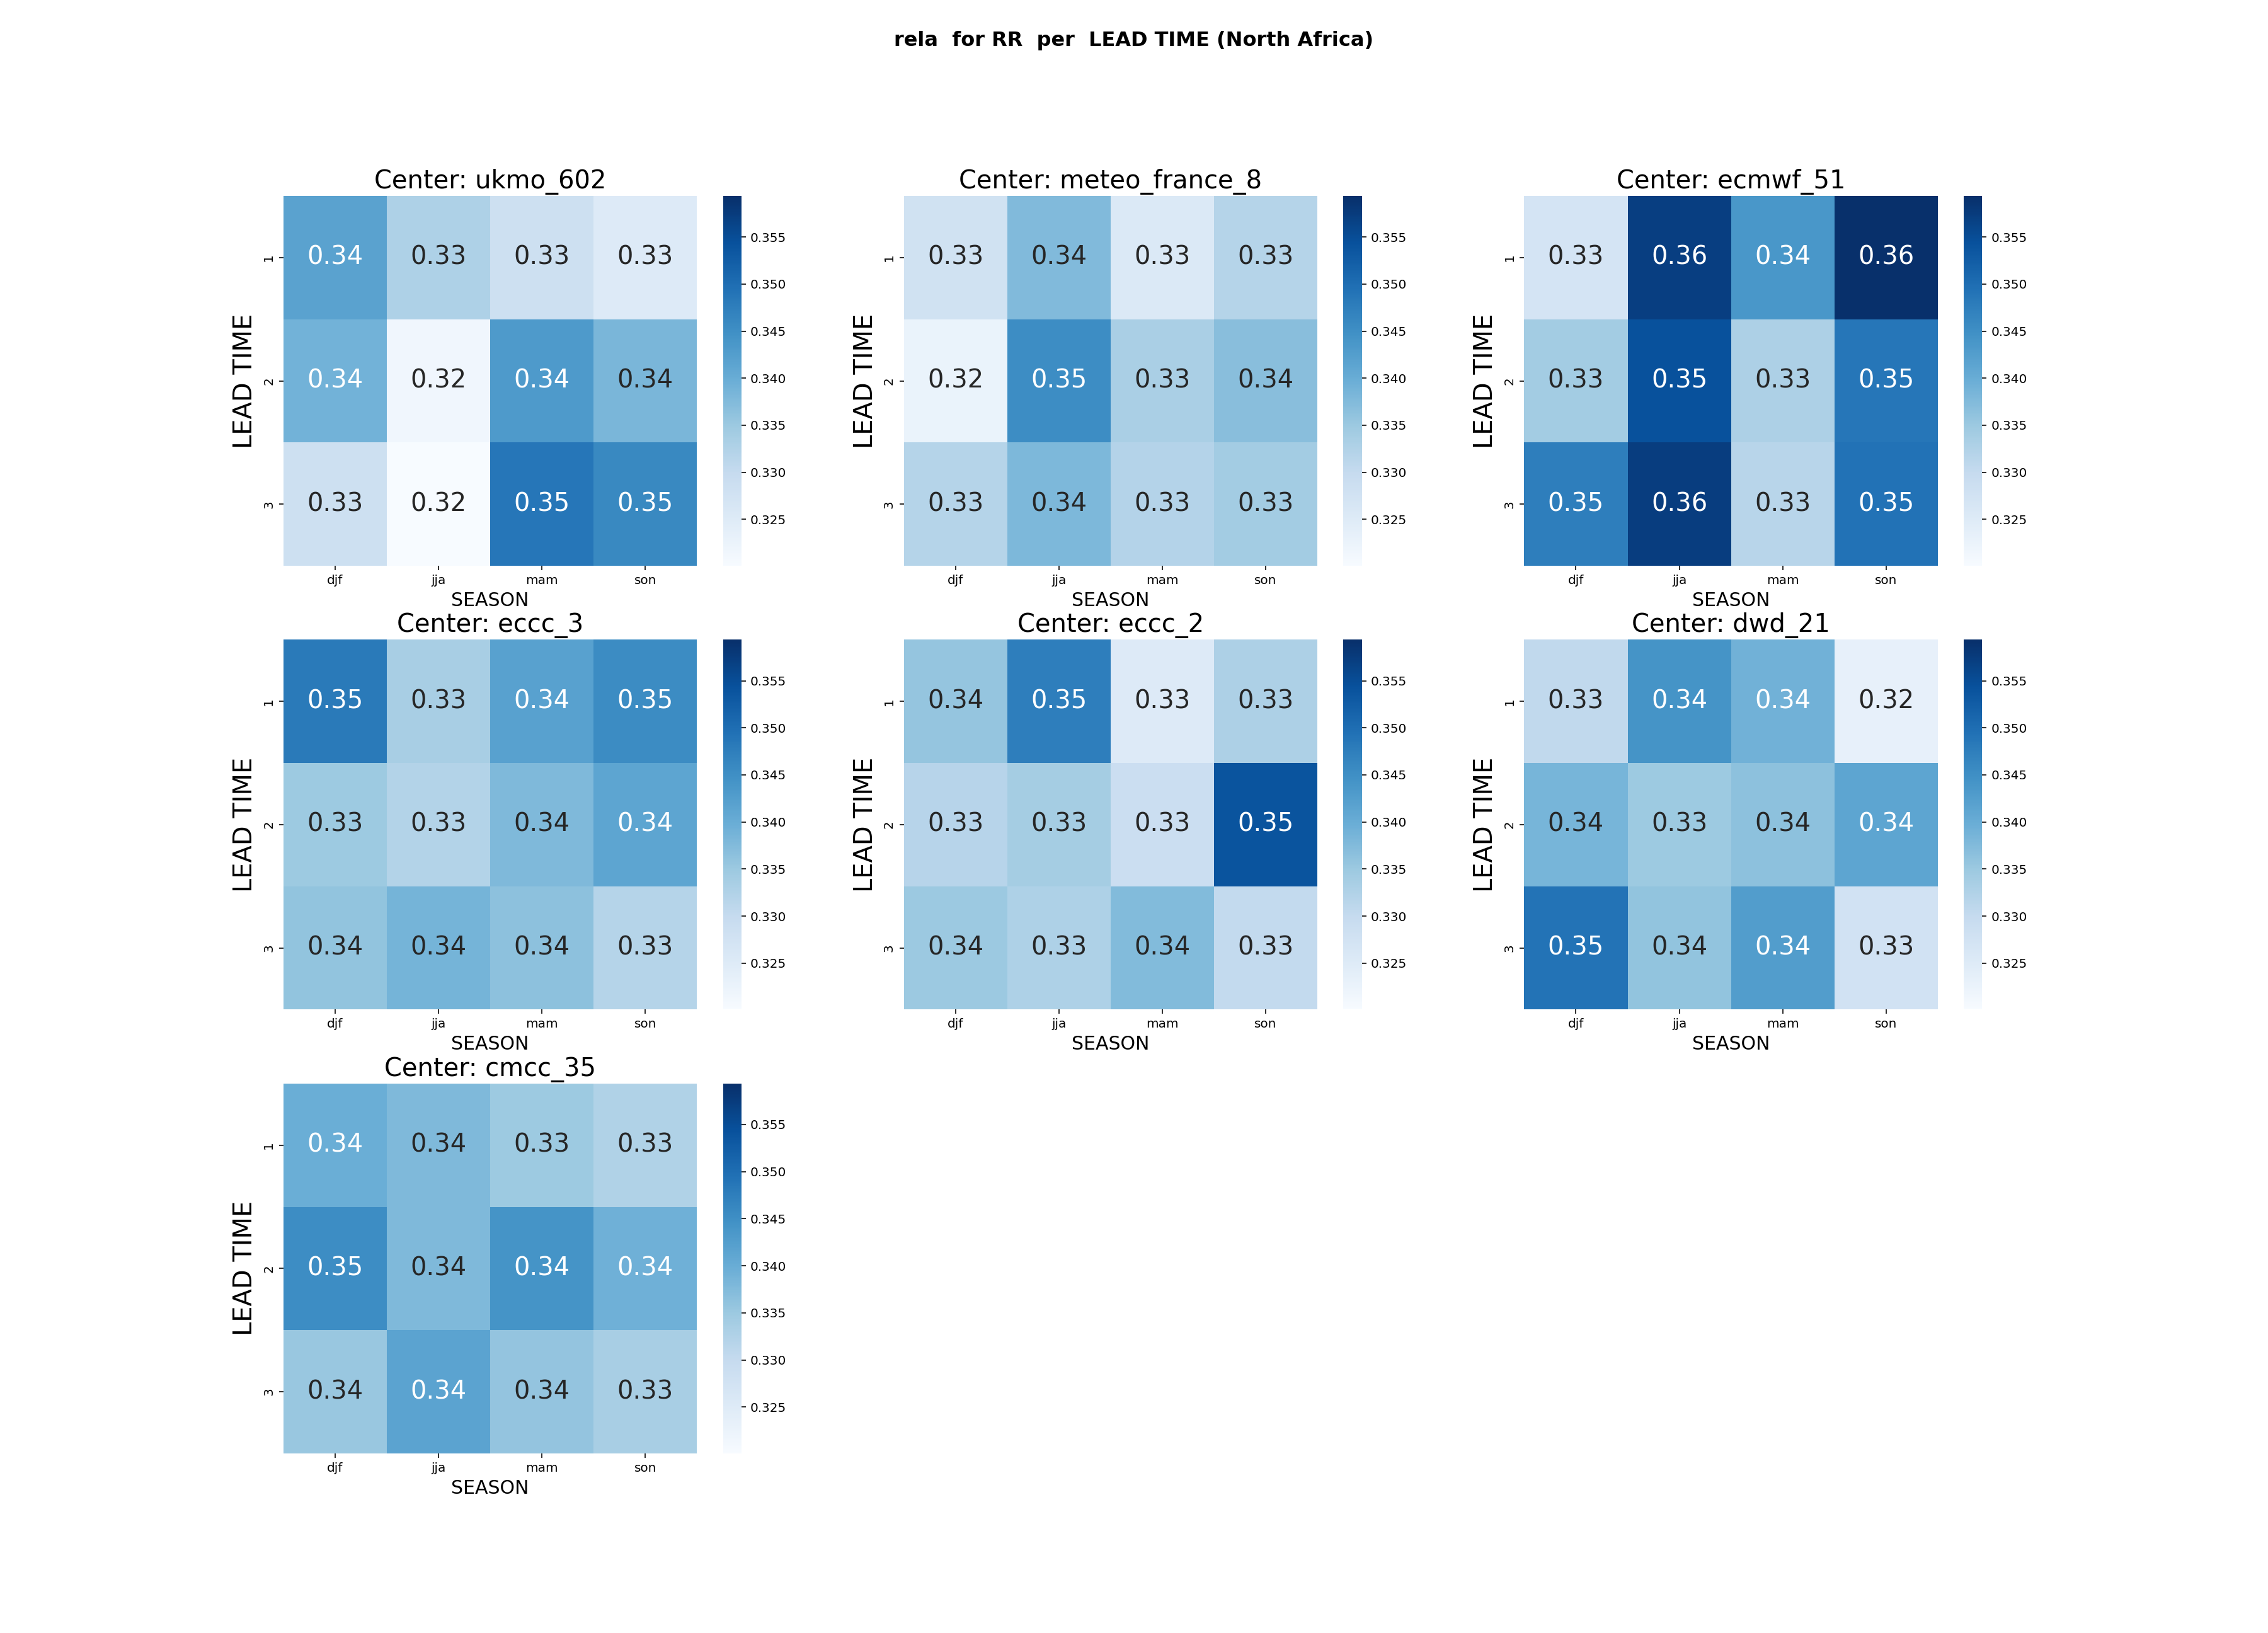
\includegraphics[scale=0.25]{plots/prob/rela/rela_RR_NorthAfrica.png}
    \caption{The Reliability Score  . \textbf{\textit{(0 means perfect Reliability)}}}
\end{figure}




\subsubsection{The ranked probability score (RPS)}


\begin{figure}[H]
    \centering
    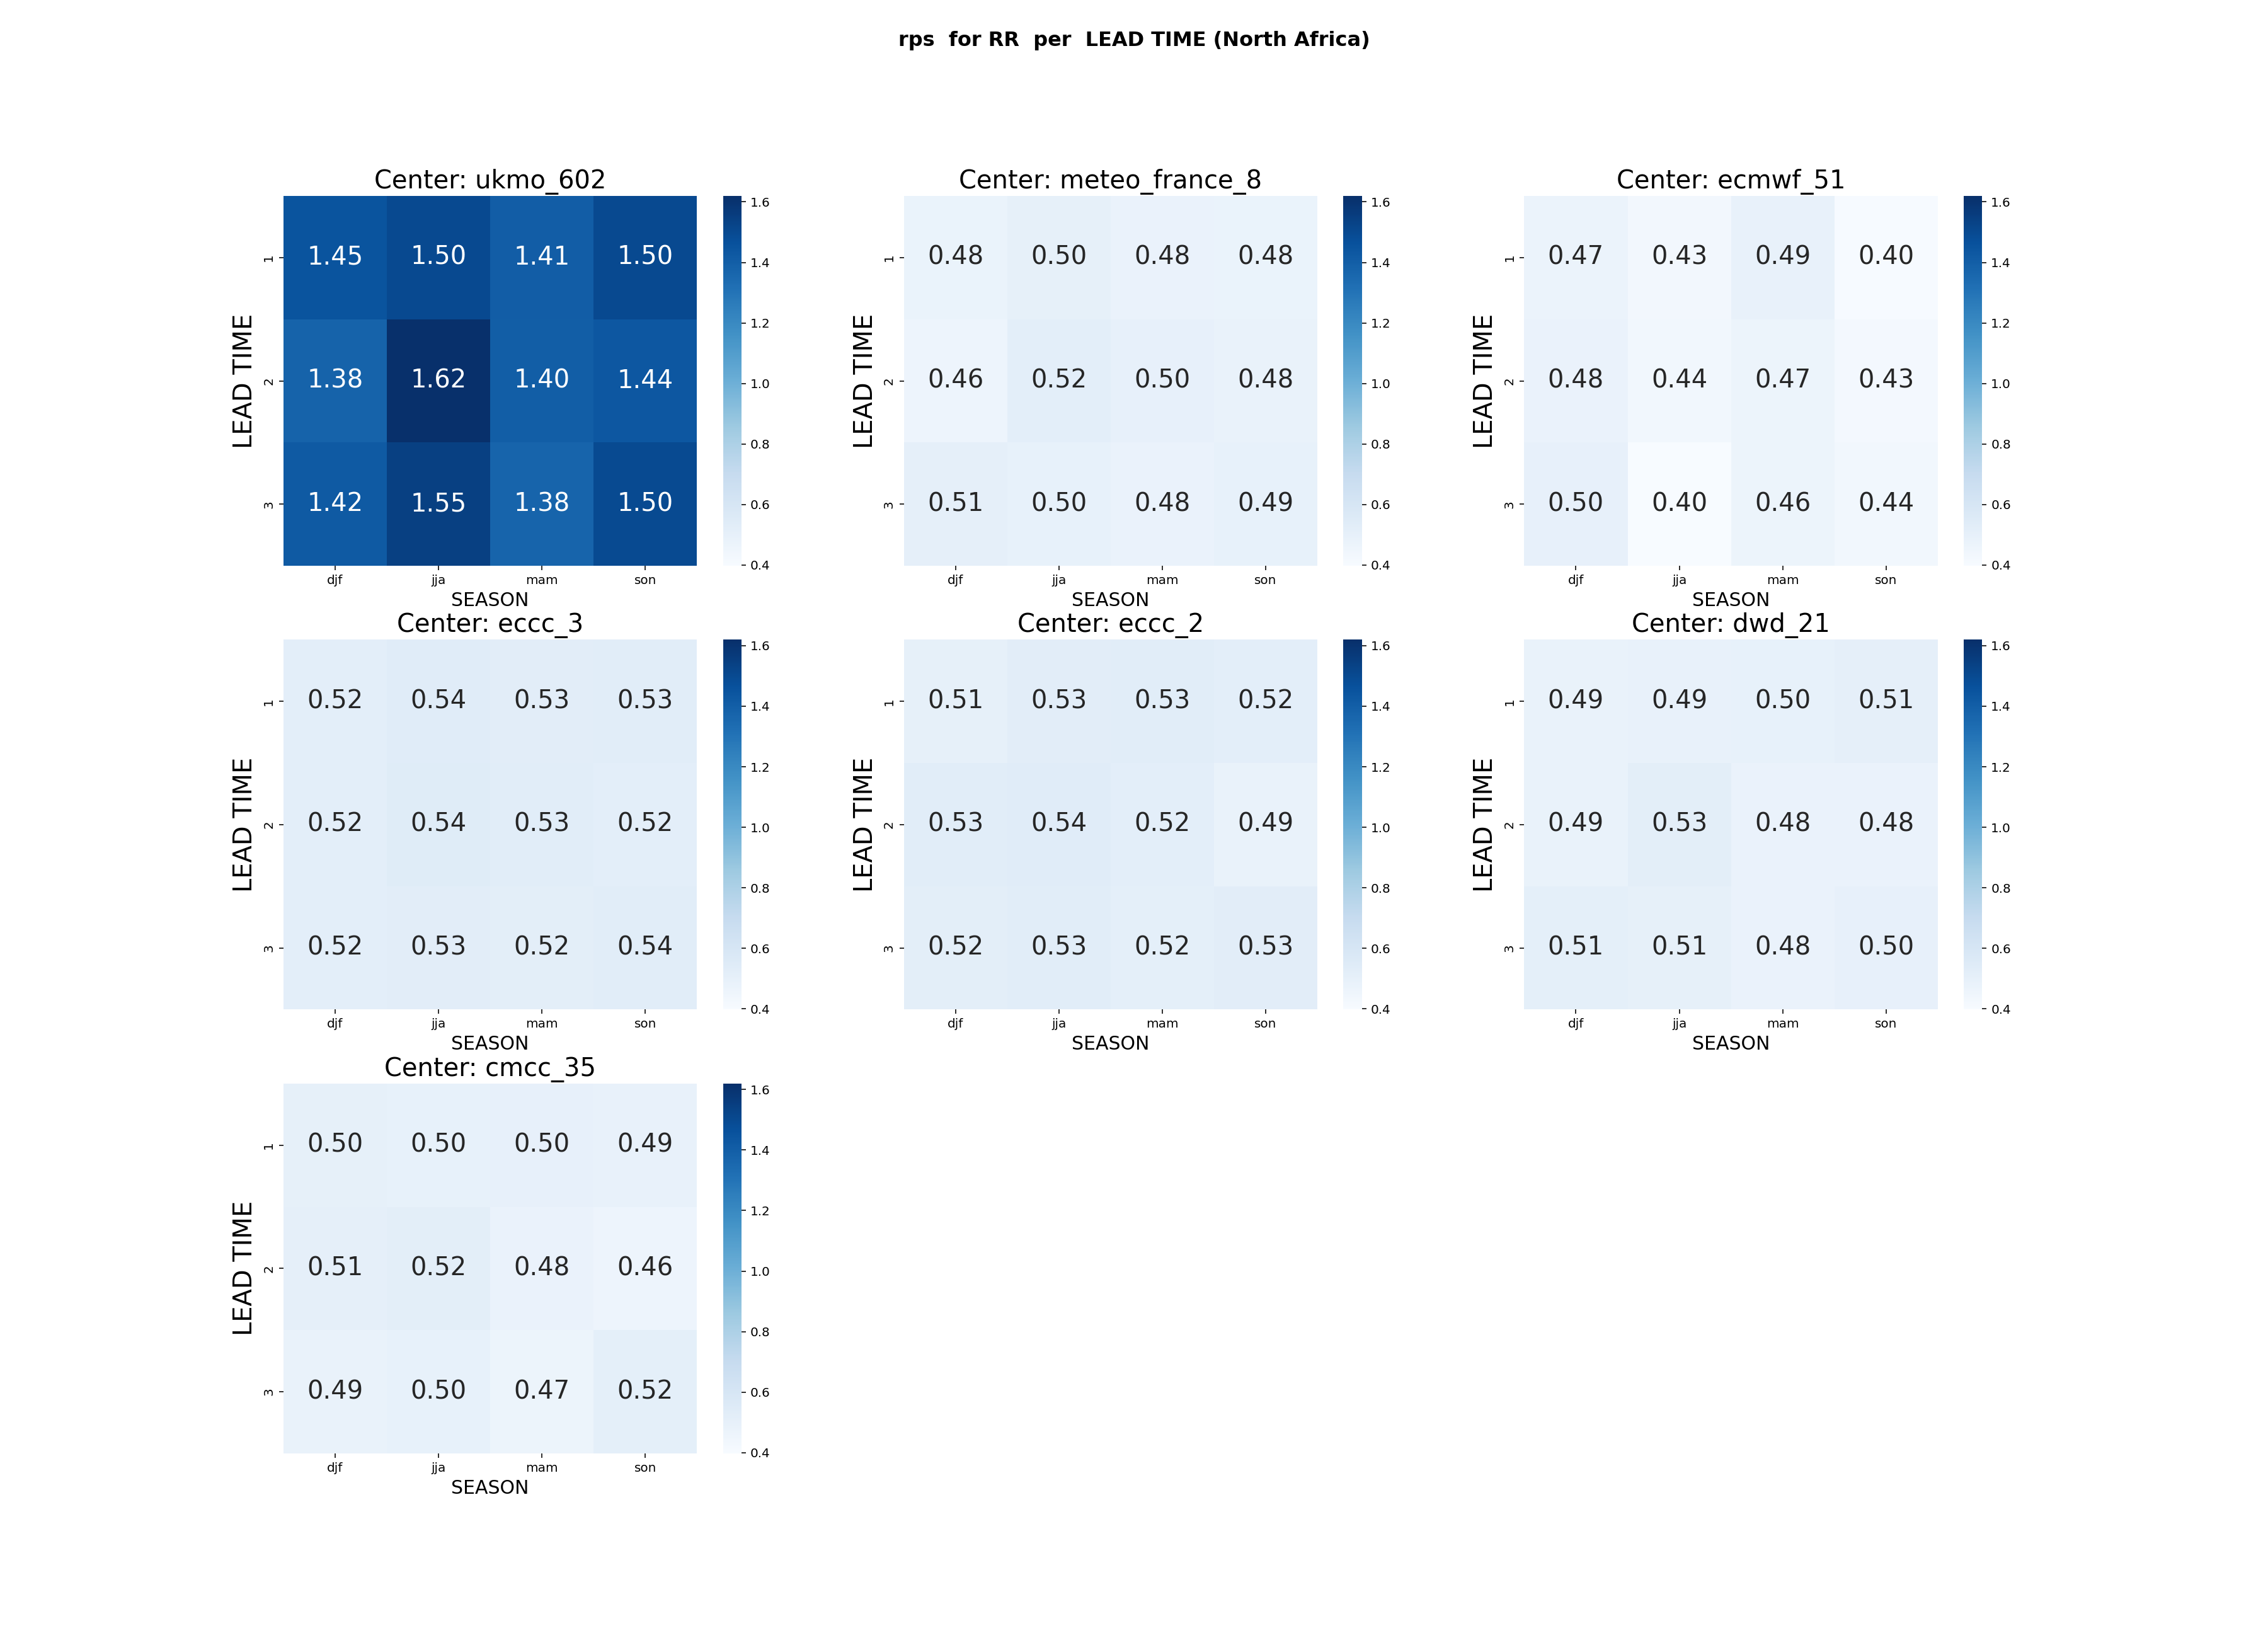
\includegraphics[scale=0.25]{plots/prob/rps/rps_RR_NorthAfrica.png}
    \caption{The Heatmap of  RPS Score on north africa region for Precipitations    . \textbf{\textit{(0 means perfect RPS)}}}
\end{figure}





\subsubsection{Relative operating characteristics}

\begin{figure}[H]
    \centering
    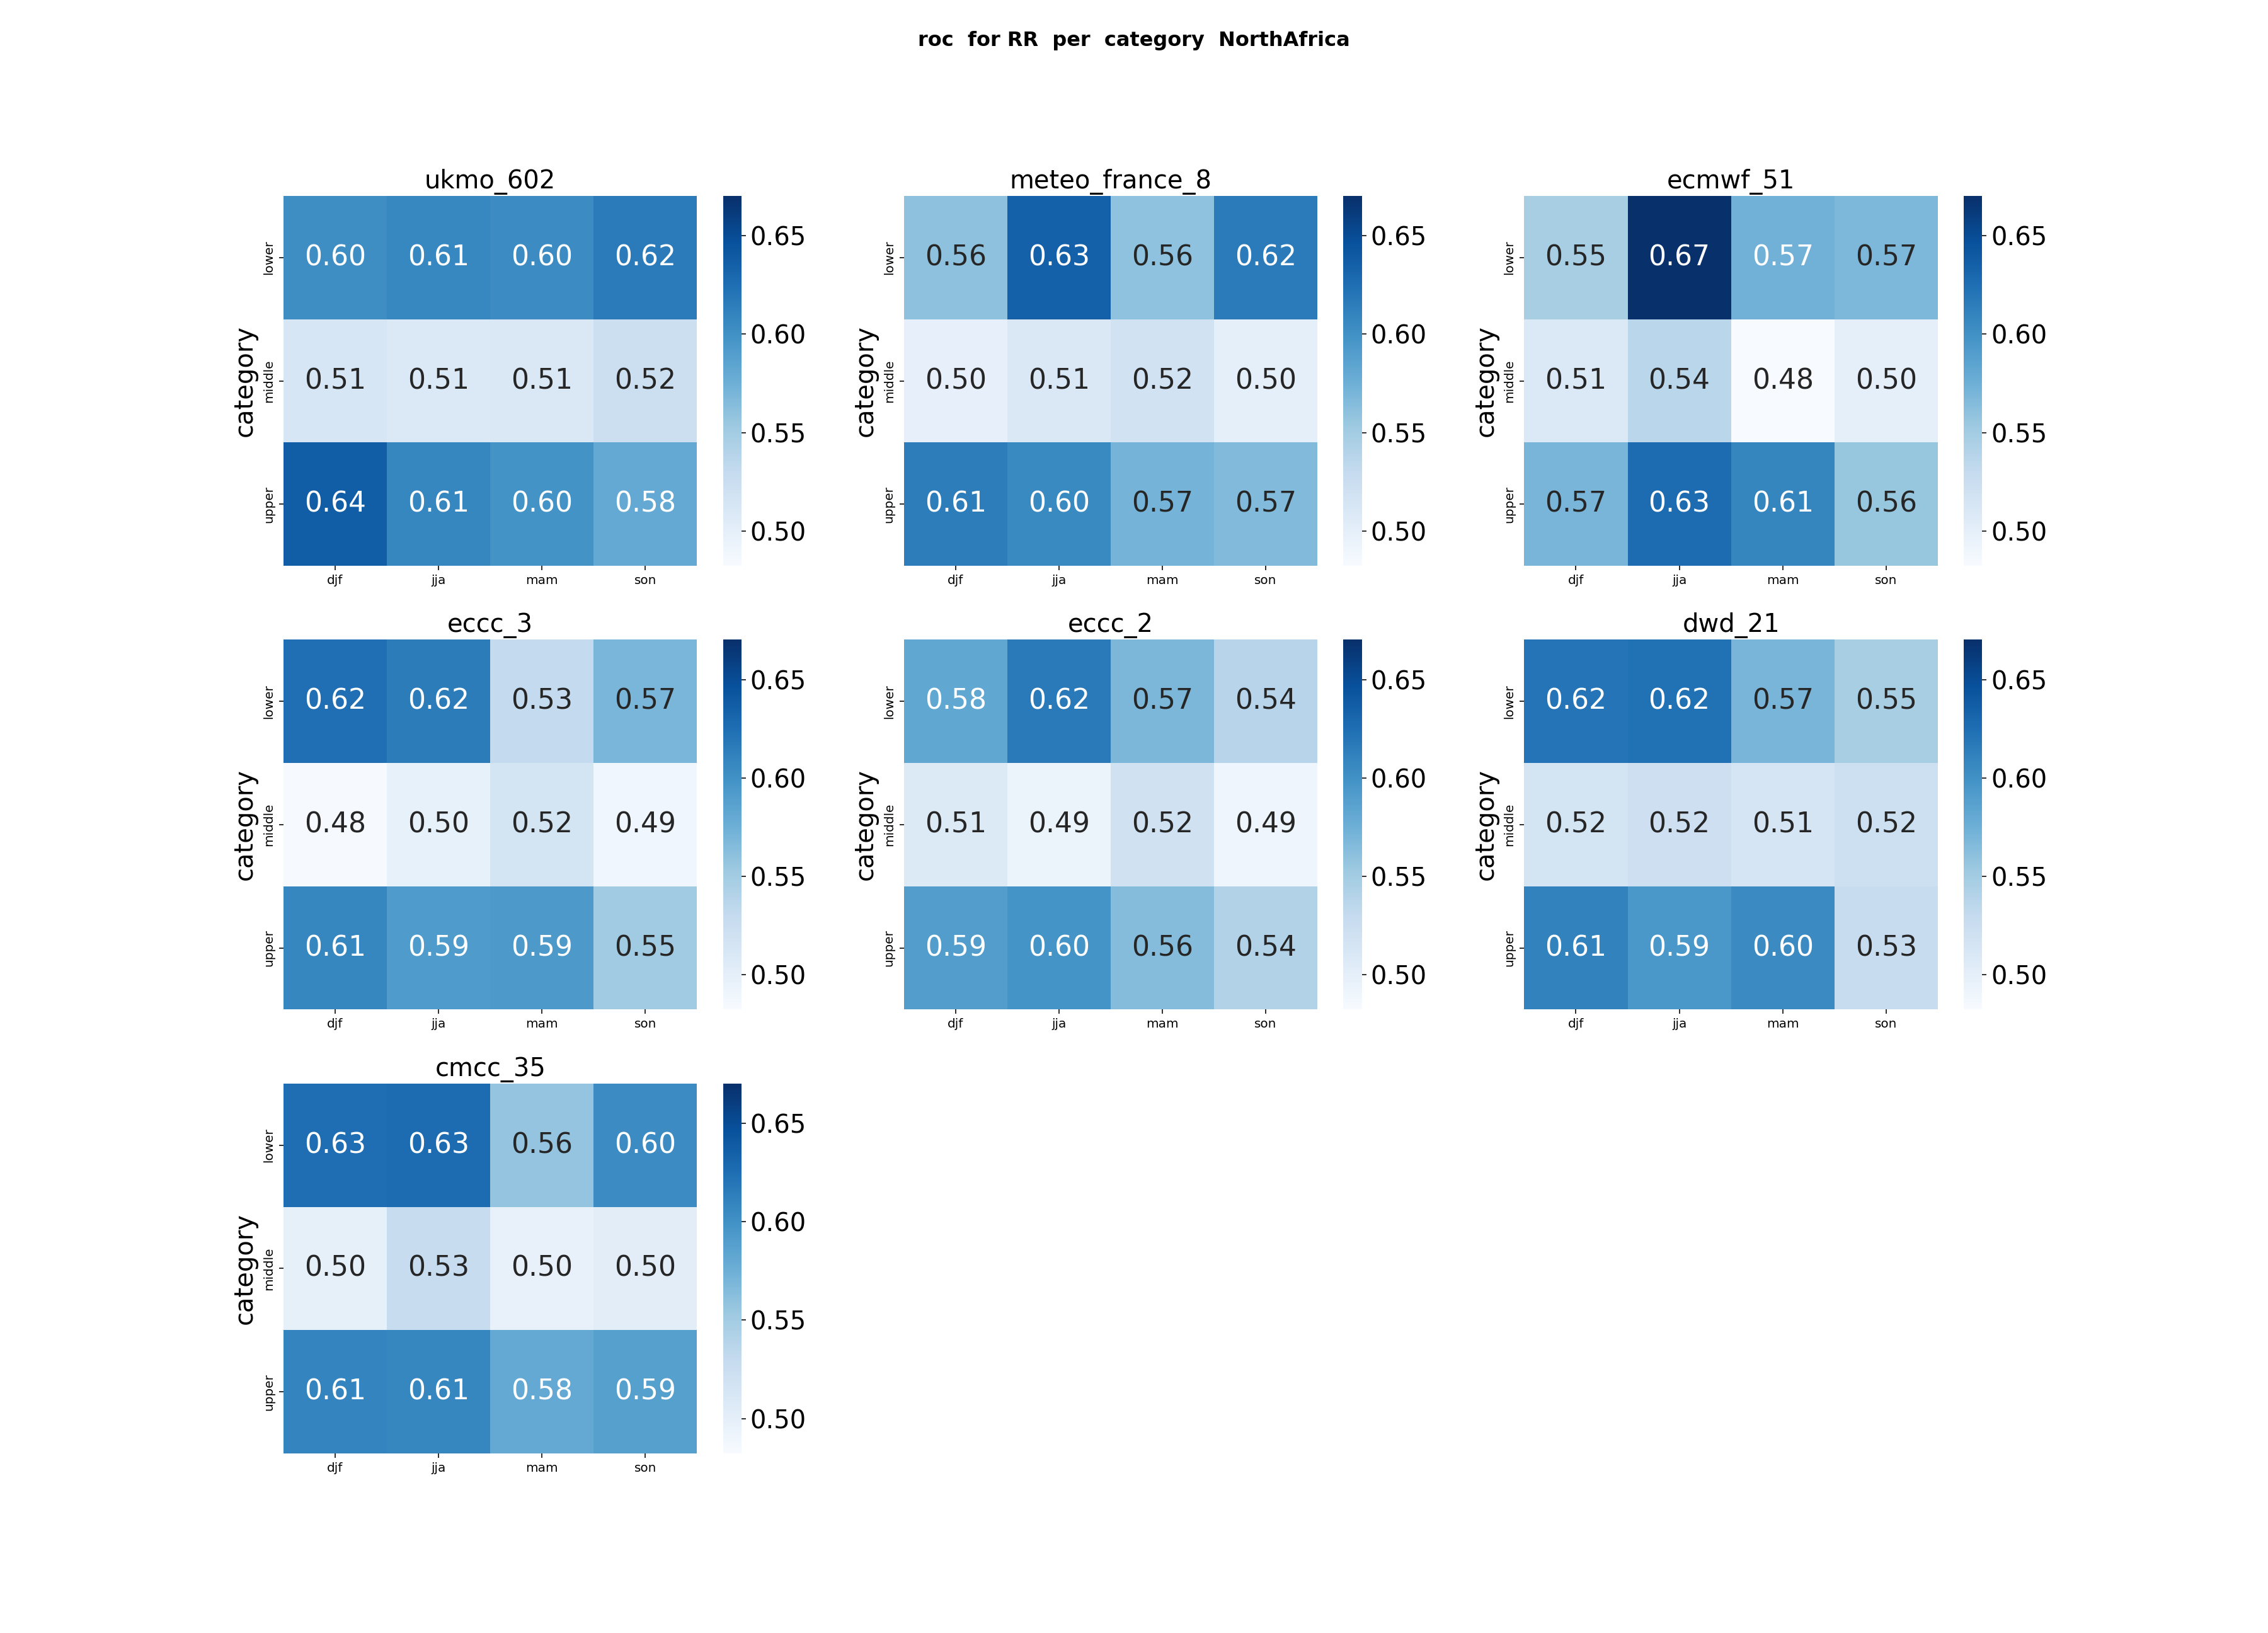
\includegraphics[scale=0.25]{plots/prob/roc/roc_RR_category_NorthAfrica.png}
    \caption{The Heatmap of ROC Score for each category  . \textbf{\textit{(1 means perfect ROC)}}}
\end{figure}

\begin{figure}[H]
    \centering
    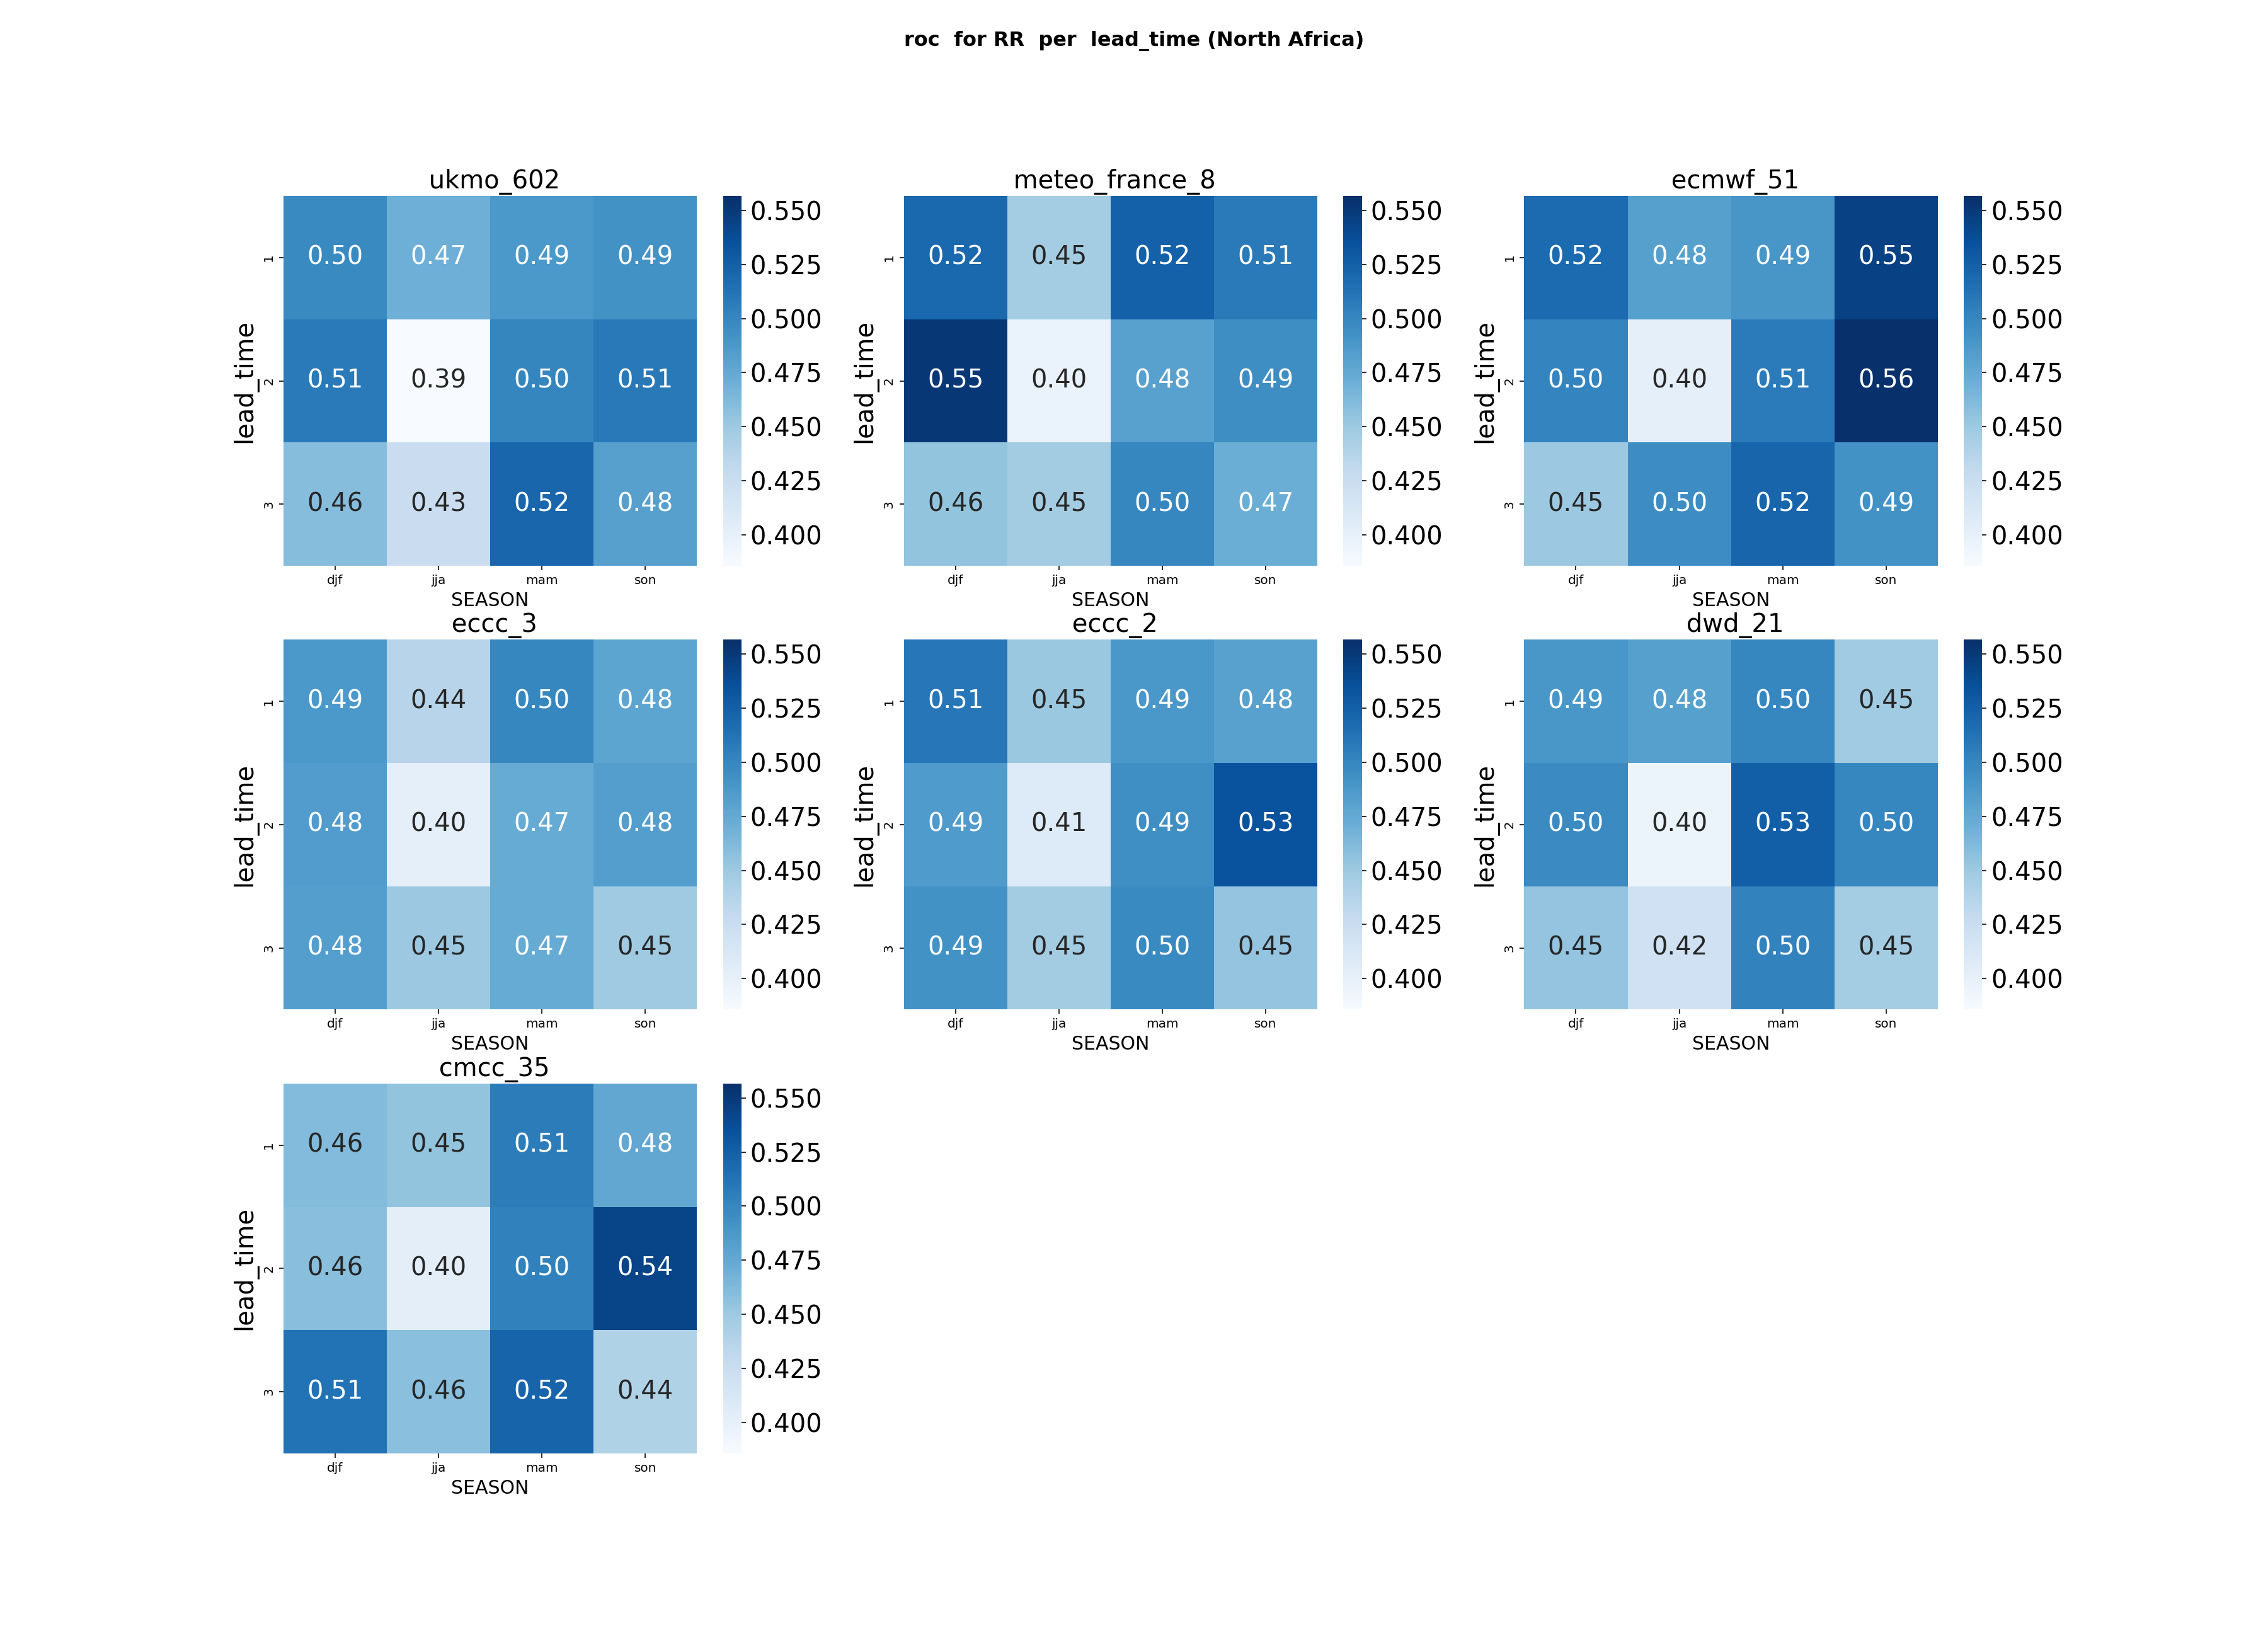
\includegraphics[scale=0.25]{plots/prob/roc/roc_RR_lead_time_NorthAfrica.png}
    \caption{The Heatmap of ROC Score for lead-times. \textbf{\textit{(1 means perfect ROC)}}}
\end{figure}



\subsubsection{Relative operating characteristics Skill Score}


\begin{figure}[H]
    \centering
    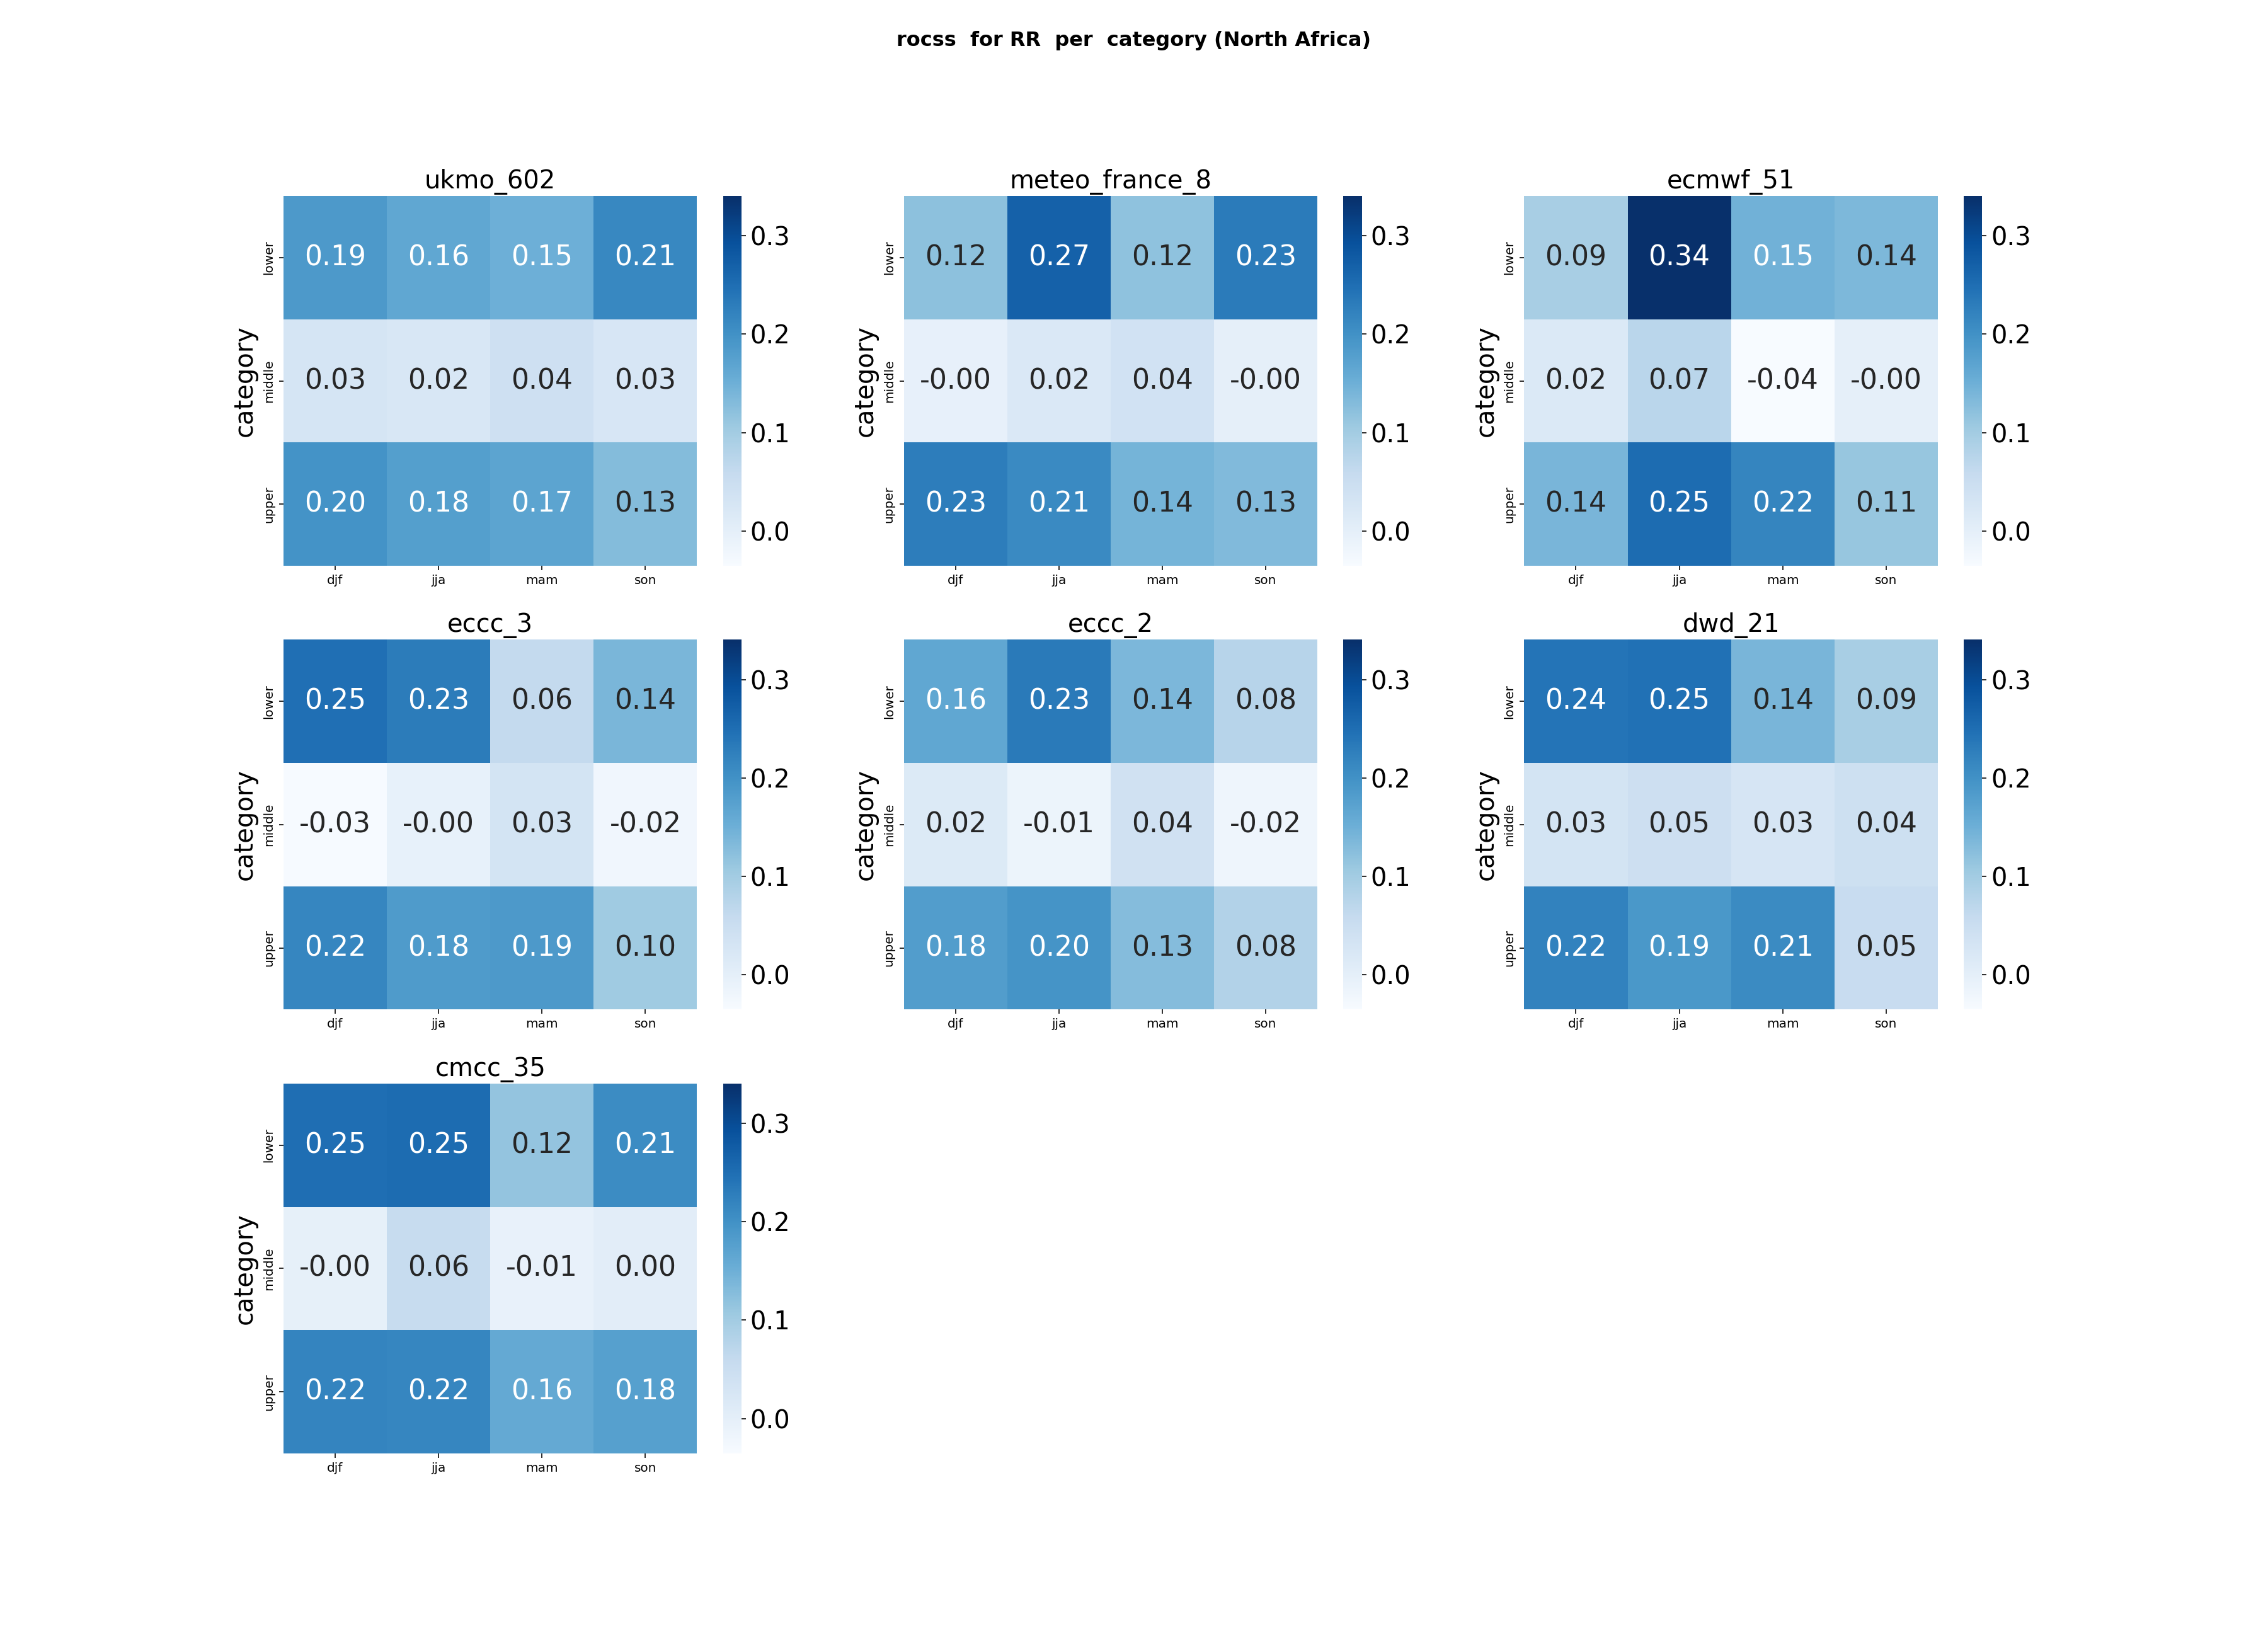
\includegraphics[scale=0.25]{plots/prob/rocss/rocss_RR_category_NorthAfrica.png}
    \caption{The ROCSS Score for each category  . \textbf{\textit{(1 means perfect ROCSS)}}}
\end{figure}


\begin{figure}[H]
    \centering
    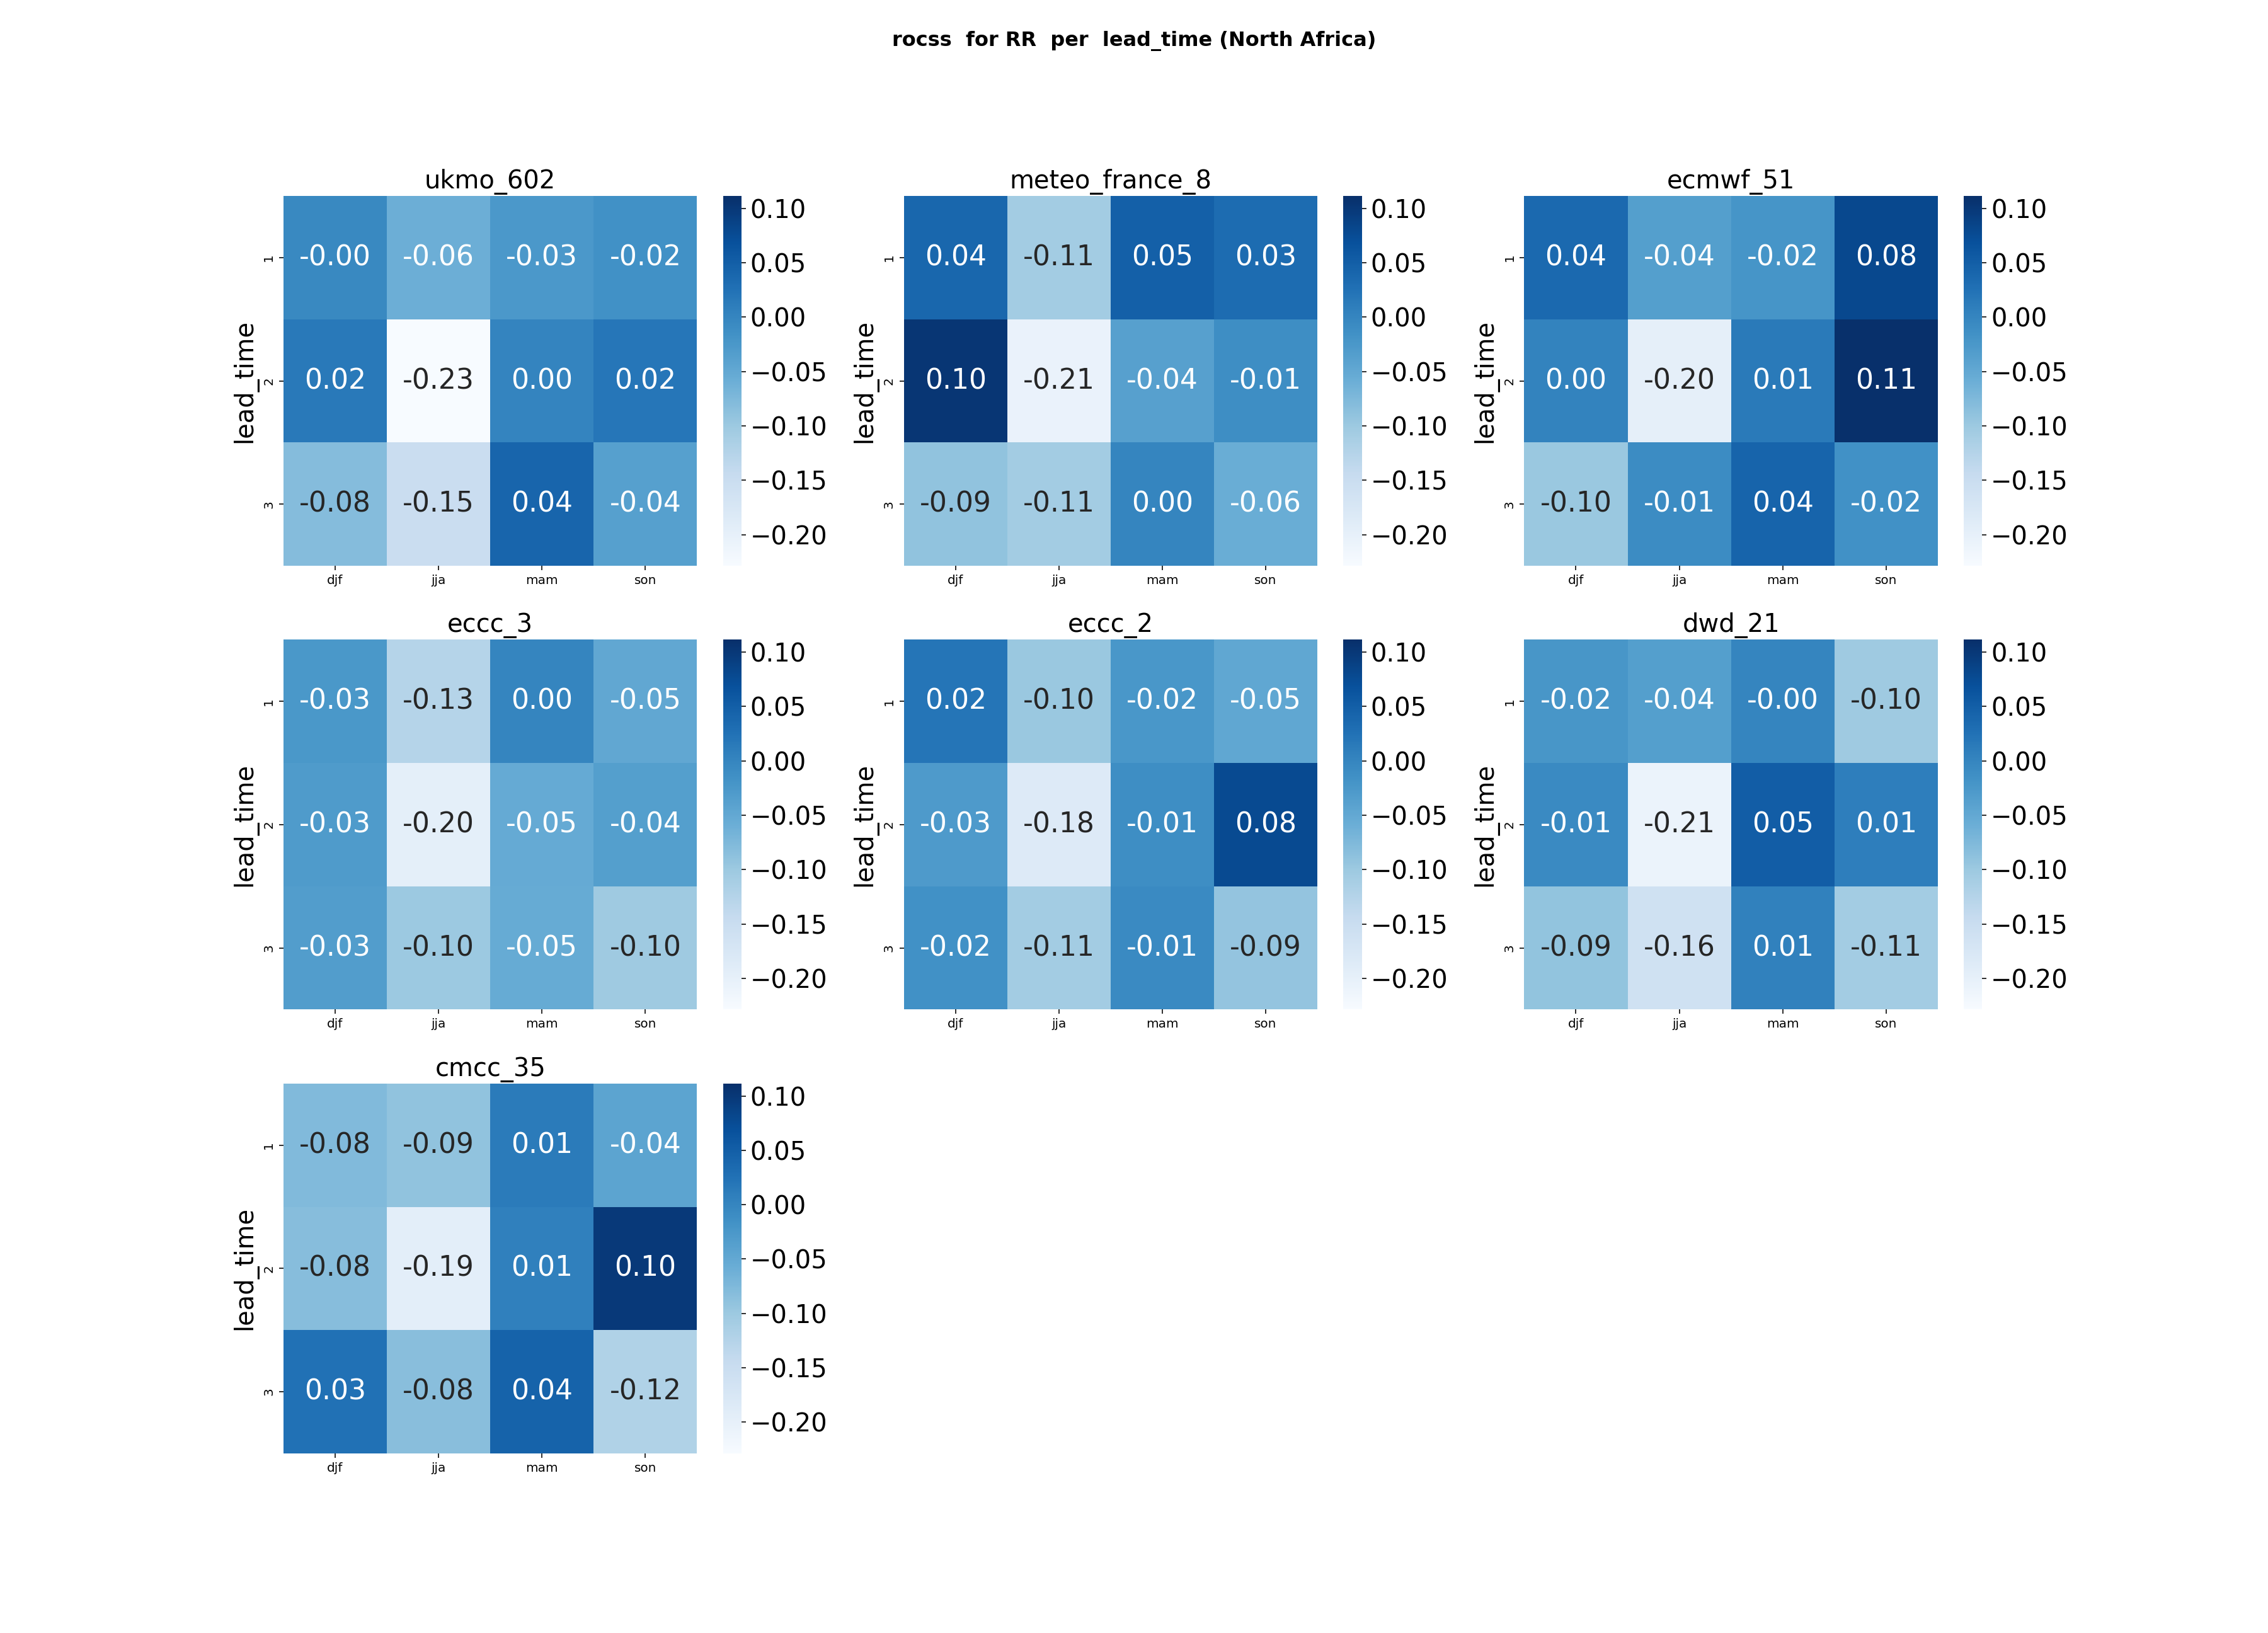
\includegraphics[scale=0.25]{plots/prob/rocss/rocss_RR_lead_time_NorthAfrica.png}
    \caption{The average of  ROCSS Score on all categories    . \textbf{\textit{(1 means perfect ROCSS)}}}
\end{figure}







